% Created 2023-09-19 火 15:51
% Intended LaTeX compiler: pdflatex
\documentclass[10pt]{article}
\usepackage[utf8]{inputenc}
\usepackage[T1]{fontenc}
\usepackage{graphicx}
\usepackage{longtable}
\usepackage{wrapfig}
\usepackage{rotating}
\usepackage[normalem]{ulem}
\usepackage{amsmath}
\usepackage{amssymb}
\usepackage{capt-of}
\usepackage{hyperref}
\usepackage[newfloat]{minted}
\usepackage[a4paper, total={6.5in, 9in}]{geometry}
\usepackage{minted}
\setminted{breaklines}
\usepackage[utf8]{inputenc}
\renewcommand{\familydefault}{\sfdefault}
\usemintedstyle{vs}
\usepackage[most]{tcolorbox}
\usepackage{CJKutf8}
\usepackage{xurl}
\usepackage{fontawesome5}
\usepackage{hyperref}
\usepackage{graphicx}
\usepackage{float}
\newcommand{\gitlab}[1]{%
\href{#1}{GitLab \faGitlab}}
\author{Vincent Conus\thanks{vincent.conus@protonmail.com}}
\date{2023-8-30}
\title{Setting up and using Xilinx KRIA KV260\\\medskip
\large \begin{CJK}{UTF8}{min}南山大学\end{CJK}}
\hypersetup{
 pdfauthor={Vincent Conus},
 pdftitle={Setting up and using Xilinx KRIA KV260},
 pdfkeywords={},
 pdfsubject={A report presenting how to use and set Xilinx's Kria board},
 pdfcreator={Emacs 30.0.50 (Org mode 9.6.6)}, 
 pdflang={English}}
\begin{document}

\begin{titlepage}
\centering
{\LARGE Setting up and using Xilinx KRIA KV260 \par }
\vspace{5mm}
{\large \begin{CJK}{UTF8}{min}南山大学\end{CJK} \par}
\vspace{1cm}
{\large 2023-8-30 \par}
\vspace{2cm}
{\large Vincent Conus -  Source available at \gitlab{https://gitlab.com/sunoc/xilinx-kria-kv260-documentation} \par}
\vspace{3cm}
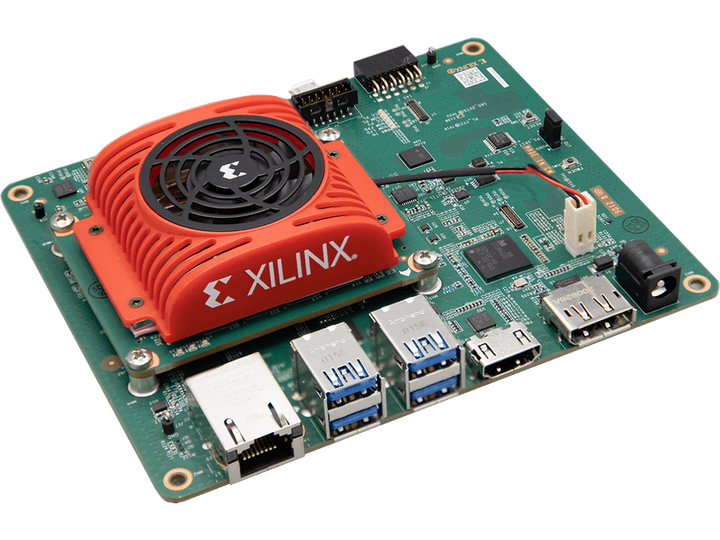
\includegraphics[width=0.8\textwidth]{./img/board}\end{titlepage}
\tableofcontents
\pagebreak
\section{Introduction \& motivation}
\label{sec:org84046b7}
This guide will present how to setup and use Xilinx's KRIA board, in particular
for running ROS on a host Ubuntu system, as well as for deploying
micro-ROS as a firmware on the MCU part of this board's chip.

The use of this device in particular is interesting because of the presence
of a CPU comprising both a general purpose ARM core, capable of running
a Linux distribution, as well as another ARM core, real-time enabled,
capable to run a RTOS. The figure \ref{fig:orgc6d7e7c} below shows a schematic
view of the overall system we are trying to archive.

\begin{figure}[htbp]
\centering
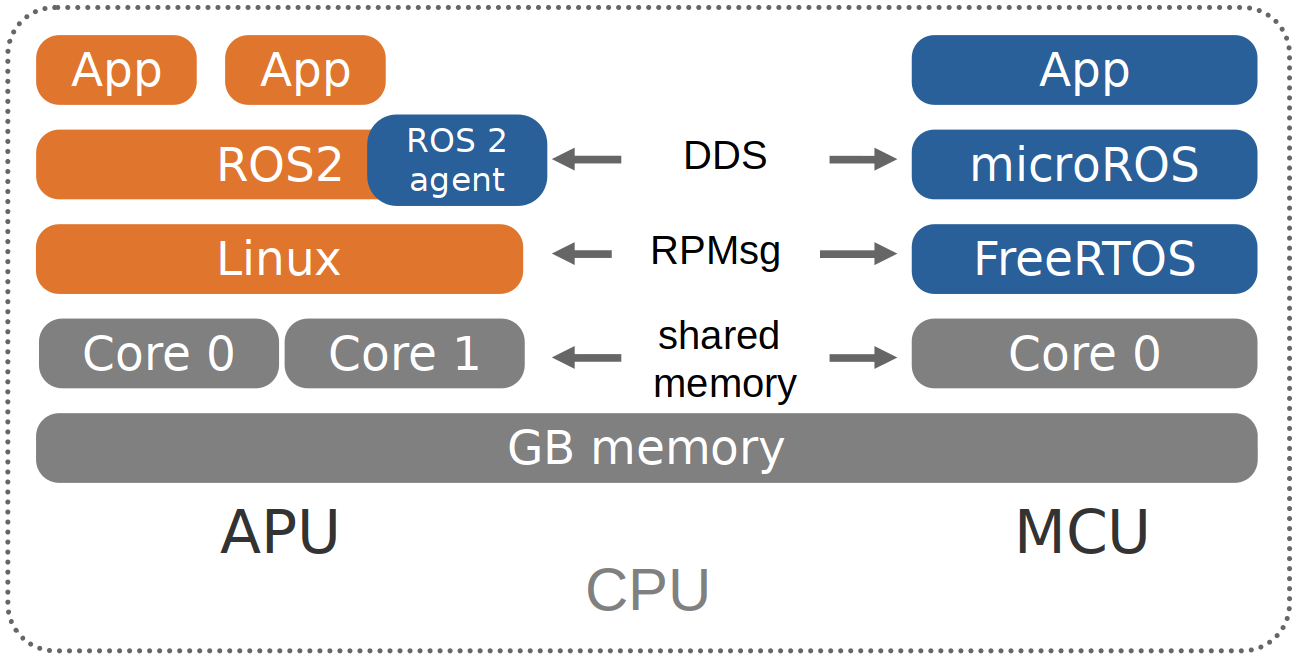
\includegraphics[width=.6\textwidth]{./img/map.png}
\caption{\label{fig:orgc6d7e7c}The Linux and ROS2 environment (orange) will communicate with the real-time, FreeRTOS and micro-ROS side (blue) using RPMsg (shared memory).}
\end{figure}

\section{Boot firmware}
\label{sec:orgfab0bc7}
The goal for the Linux side of the deployment is to
have the latest LTS version of Ubuntu up and running.

In order to be able to boot such a newer version of Linux, the
boot image of the board must first be updated.

The procedure is available in \href{https://docs.xilinx.com/r/en-US/ug1089-kv260-starter-kit/Firmware-Update}{the official documentation},
but I will present it step by step here.

\subsection{Getting the new firmware}
\label{sec:org75a32cf}
A 2022 version of the board firmware is required in order to run the latest
version of Ubuntu properly.

The image can be downloaded at \href{https://xilinx-wiki.atlassian.net/wiki/spaces/A/pages/1641152513/Kria+K26+ SOMoot-FW-update-with-xmutil}{the atlassian page} on the topic,
or even directly with the following command:

\begin{minted}[frame=single,framesep=2mm,baselinestretch=1.2,linenos,breaklines,fontsize=\footnotesize]{sh}
wget https://www.xilinx.com/member/forms/download/\
     design-license-xef.html?filename=BOOT-k26-starter-kit-20230516185703.bin
\end{minted}


\subsection{Reaching the board recovery tool}
\label{sec:org404b7e6}
Now the firmware \texttt{.bin} image is available, it is possible to update it using the
boards recovery tool. Here are the steps that must be taken in order to reach
this tool and update the board:

\begin{itemize}
\item Connect the board to your machine via a Ethernet cable.
This will obviously cut you internet access, so you should be set for that.
\item Select the wired network as your connection (must be "forced", since it
doesn't have internet access).
\item Set a fixed IP address for your machine, in the \texttt{192.168.0.1/24}
range, except the specific \texttt{192.168.0.111}, which will be used by the
board.
The netmark and gateway should also be respectively set to
\texttt{255.255.255.0} and \texttt{192.168.0.1}.
\item Hold the firmware update button (FWUEN) when powering back the board.
\item Using a web browser on your host machine, access
\texttt{http://192.168.0.111}. Thou shall now see the interface, as visible on
the figure \ref{fig:orgcd772cd} below. If the page struggle to appear,
\end{itemize}
you should try to un-plug and re-plug the Ethernet cable.

\begin{figure}[htbp]
\centering
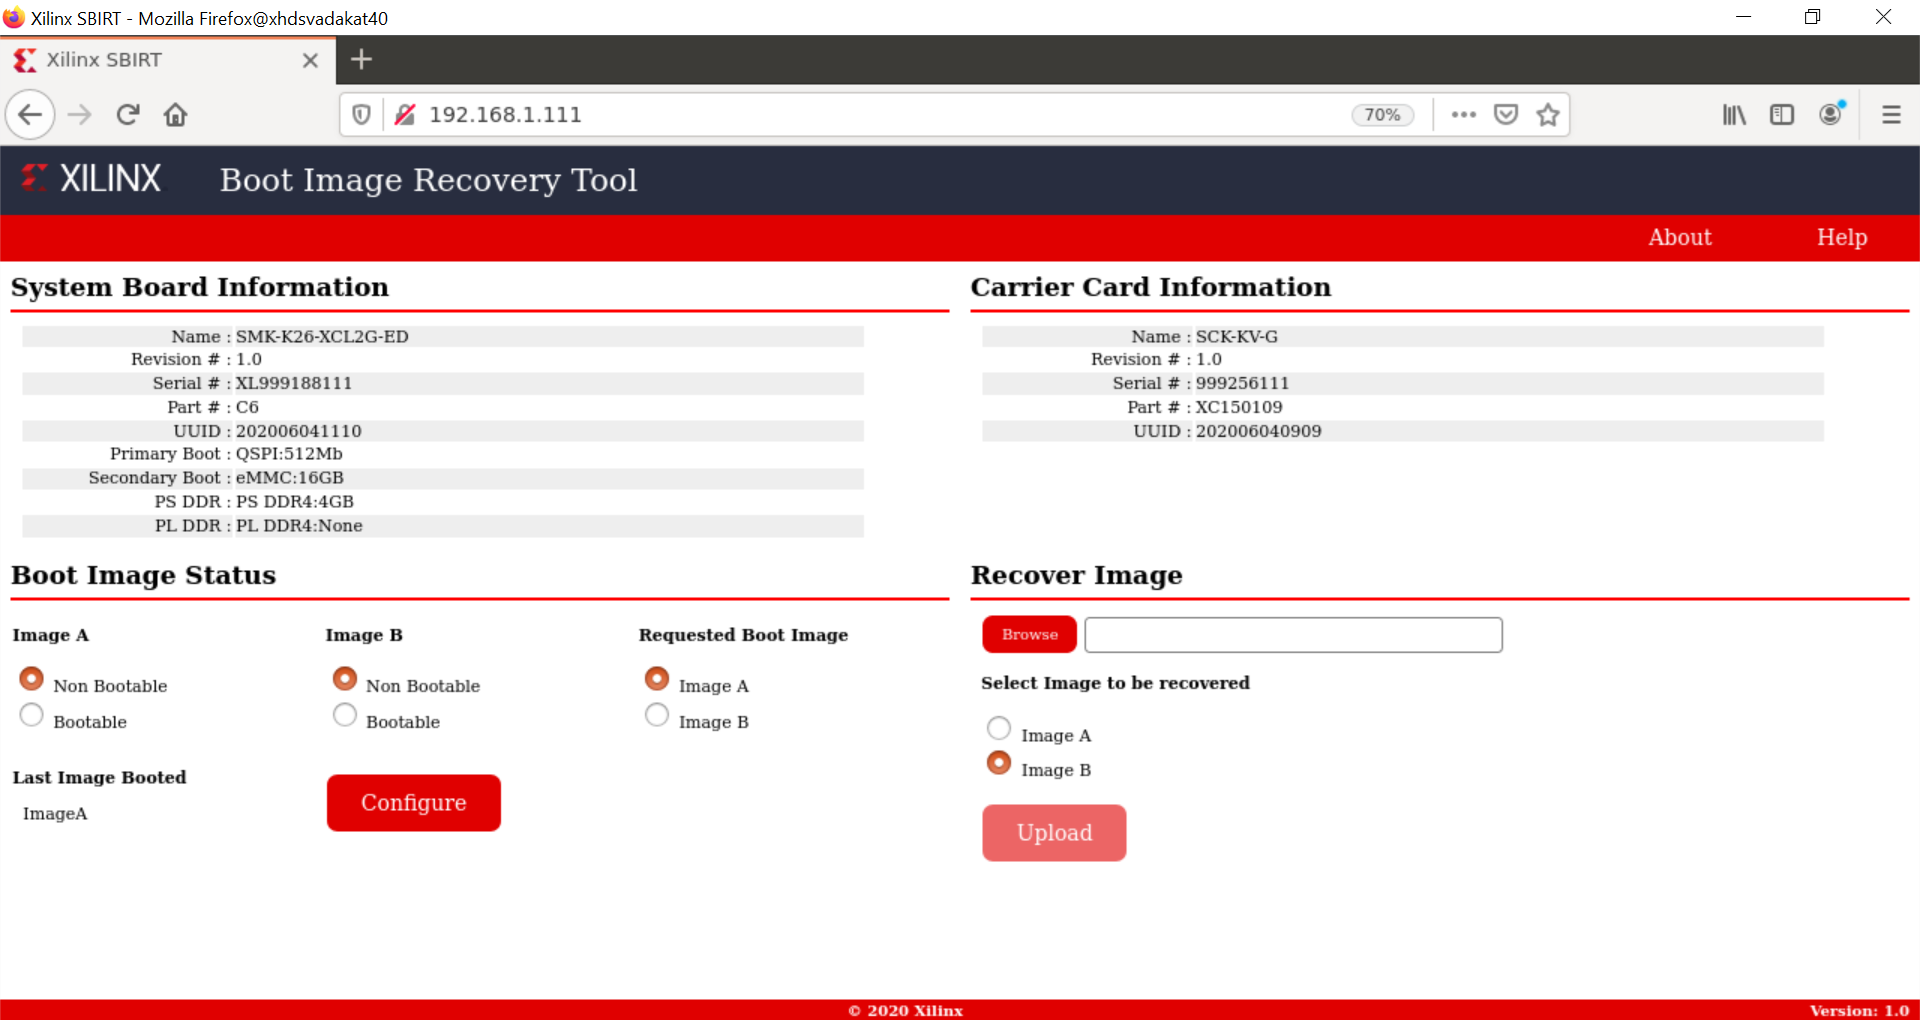
\includegraphics[width=1\textwidth]{img/recovery.png}
\caption{\label{fig:orgcd772cd}The recovery tool for the board, access from Firefox. We can see board information at the center, and the tools to upload the firmware at the bottom of the page.}
\end{figure}

\subsection{Updating the boot firmware}
\label{sec:org1da19bf}
From this "recovery" page, it is possible to upload the \texttt{.bin} file downloaded previously onto
the board using the "Recover Image" section at the bottom right of the page.

The board can be re-booted afterwards.
\pagebreak

\section{Installing Linux}
\label{sec:org124fdad}
Withe the boot firmware being up-to-date, we can proceed to install a Linux distribution
on our Kria board. The step needed to archive a full installation of Ubuntu LTS 22.04
will be presented in this section\footnote{The same procedure should work for other versions of Ubuntu, as long as they
support the Kria board, but for this report and project, only the LTS 22.04 was tested
(as of 2023-08-30).}. The figure \ref{fig:org28f64b5} below shows
where this operating system sits in the general system we are implementing.

\begin{figure}[htbp]
\centering
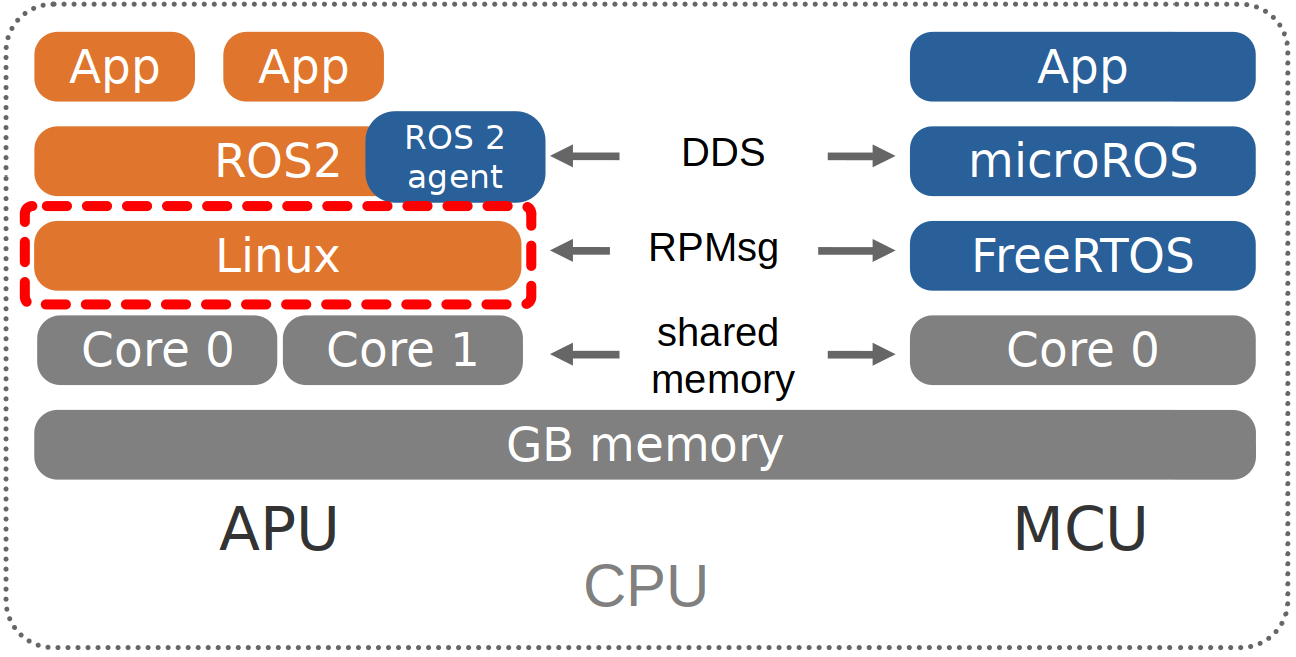
\includegraphics[width=.6\textwidth]{./img/map_linux.png}
\caption{\label{fig:org28f64b5}The Linux operating system (red border)runs on the APU (application, general purpose) side of the Kria board CPU. It is the base layer for the ROS2 system.}
\end{figure}

\subsection{Preparing and booting a Ubuntu 22.04 media}
\label{sec:orgb915bc5}
An \href{https://ubuntu.com/download/amd-xilinx}{official Ubuntu image} exists and is
provided by Xilinx, allowing the OS installation to be quick and
straightforward.
Ubuntu is a common and easy to use distribution. Furthermore,
it allows to install ROS2 as a package, which is most convenient and will be
done later in this guide.

Once the image has been downloaded at \href{https://ubuntu.com/download/amd-xilinx}{Canonical's page}
we can flash it onto the SD card, with the following instructions.

\begin{tcolorbox}[colback=red!5!white,colframe=red!75!black]
\textbf{DANGER}: The next part involve the \texttt{dd} command writing on disks!!!
As always with the dd command, thou have to be \textbf{VERY} careful on what arguments
thou give. Selecting the wrong disk will result on the destruction of
thy data !!
\uline{If you are unsure of what to do, seek assistance !}
\end{tcolorbox}

With the image available on thy machine and a SD card visible as \texttt{/dev/sda} device\footnote{Again, it is \uline{critical} to be 100$\backslash$% certain that you are working with
the correct device!}
one can simply run the \texttt{dd} command as follow to write the image to a previously formatted drive (here \texttt{/dev/sda}):

\begin{minted}[frame=single,framesep=2mm,baselinestretch=1.2,linenos,breaklines,fontsize=\footnotesize]{sh}
unxz iot-limerick-kria-classic-desktop-2204-x07-20230302-63.img.xz
sudo dd if=iot-limerick-kria-classic-desktop-2204-x07-20230302-63.img \
     of=/dev/sda status=progress bs=8M && sync
\end{minted}


Once the SD card is flashed and put back in the board, the micro-USB cable can be
connected from the PC to the board. It is then possible to
connect to the board in serial with an appropriate tool, for example \texttt{picocom},
as in the following example (the serial port that "appeared" was the \texttt{/dev/ttyUSB1} in this case,
and the 115200 bitrate is the default value for the board):

\begin{minted}[frame=single,framesep=2mm,baselinestretch=1.2,linenos,breaklines,fontsize=\footnotesize]{sh}
sudo picocom /dev/ttyUSB1 -b 115200
\end{minted}

Once logged in, it is typically easier and more convenient to connect the board
using SSH. When the board is connected to the network, it is possible to know
it's IP address with the \texttt{ip} command; then it is possible to connect to
the board with ssh, as follow (example, with the first command to be run on the board
and the second one on the host PC, both without the first placeholder hostnames):


\begin{minted}[frame=single,framesep=2mm,baselinestretch=1.2,linenos,breaklines,fontsize=\footnotesize]{sh}
kria# ip addr

host# ssh ubuntu@192.168.4.11
\end{minted}

\subsection{Network and admin setups}
\label{sec:orga8f6e0f}
This section presents a variety of extra convenience configurations
that can be used when setting-up the Kria board.

\subsubsection{Proxy and DNS}
\label{sec:orgb8d3d37}
An issue that can occur when connecting the board to the internet is the
conflicting situation with the university proxy.
Indeed, as the network at Nanzan University requires to go through a proxy,
some DNS errors appeared.

Firstly, it is possible to set a DNS IP address in \texttt{/etc/resolv.conf} by
editing it and adding your favorite DNS, for example \texttt{nameserver 1.1.1.1}
next to the other \texttt{nameserver} entry. The resolver can then be restarted.

\begin{minted}[frame=single,framesep=2mm,baselinestretch=1.2,linenos,breaklines,fontsize=\footnotesize]{sh}
sudo nano /etc/resolv.conf

sudo systemctl restart systemd-resolved
\end{minted}

Secondly, it might become needed to setup the proxy for the school.

This can be done as follow, by exporting a https base proxy configuration
containing you AXIA credentials (this is specific to Nanzan University IT system),
then by consolidating the configuration for other types of connections in the \texttt{bashrc}:

\begin{minted}[frame=single,framesep=2mm,baselinestretch=1.2,linenos,breaklines,fontsize=\footnotesize]{sh}
export https_proxy="http://<AXIA_username>:\
       <AXIA_psw>@proxy.ic.nanzan-u.ac.jp:8080"

echo "export http_proxy=\""$https_proxy"\"" >> ~/.bashrc \
     echo "export https_proxy=\""$https_proxy"\"" >> ~/.bashrc \
     echo "export ftp_proxy=\""$https_proxy"\"" >> ~/.bashrc \
     echo "export no_proxy=\"localhost, 127.0.0.1,::1\"" \
     >> ~/.bashrc
\end{minted}

Eventually the board can be rebooted in order for the setup to get applied cleanly.

\subsubsection{\texttt{root} password}
\label{sec:org62b83d2}
\begin{tcolorbox}[colback=orange!5!white,colframe=orange!75!black]
\textbf{WARNING}: Depending on your use-case, the setup presented in this
subsection can be a critical security breach as it remove the need for a root
password to access the admin functions of the board's Linux.
\uline{When in doubt, do not apply this configuration!!}
\end{tcolorbox}

If you board does not hold important data
and is available to you only, for test or development,
it might be convenient for the \texttt{sudo} tool to not ask for the
password all the time.
This change can be done by editing the sudoers file, and
adding the parameter \texttt{NOPASSWD}
at the \texttt{sudo} line:

\begin{minted}[frame=single,framesep=2mm,baselinestretch=1.2,linenos,breaklines,fontsize=\footnotesize]{sh}
sudo visudo

%sudo   ALL=(ALL:ALL) NOPASSWD: ALL
\end{minted}

Again, this is merely a convenience setup for devices staying at you desk. If
the board is meant to be used in any kind of production setup, a password
should be set for making administration tasks.

With all of these settings, you should be able to update the software of your
board without any issues:
\begin{minted}[frame=single,framesep=2mm,baselinestretch=1.2,linenos,breaklines,fontsize=\footnotesize]{sh}
sudo apt-get update
sudo apt-get dist-upgrade
sudo reboot now
\end{minted}


\subsubsection{Static IP address}
\label{sec:orgc79a949}
A static IP can be set by writing the following
configuration into your \texttt{netplan} configuration file.

The name of the files might vary:
\begin{minted}[frame=single,framesep=2mm,baselinestretch=1.2,linenos,breaklines,fontsize=\footnotesize]{sh}
sudo nano /etc/netplan/50-cloud-init.yaml
\end{minted}

You can then set the wanted IP as follow. Note that a custom DNS was
also set in that case.
\begin{minted}[frame=single,framesep=2mm,baselinestretch=1.2,linenos,breaklines,fontsize=\footnotesize]{yaml}
network:
  renderer: NetworkManager
  version: 2
  ethernets:
    eth0:
      addresses:
        - 192.168.11.103/24
      routes:
        - to: default
          via: 192.168.11.1
      nameservers:
        addresses:
          - 8.8.8.8
          - 1.1.1.1
\end{minted}

Finally, the change in settings can be applied
as follow:

\begin{minted}[frame=single,framesep=2mm,baselinestretch=1.2,linenos,breaklines,fontsize=\footnotesize]{sh}
sudo netplan apply
\end{minted}

\subsubsection{Purging \texttt{snap}}
\label{sec:orgd487cc7}
As the desktop-specific software are not used at all in the case
of our project, there are some packages that can be purges in order for the
system to become more lightweight.

In particular, the main issue with Ubuntu systems is the forced integration of
Snap packages. Here are the command to use in order to remove all of that.
These steps take a lot of time and need to be executed in that specific order\footnote{The \texttt{snap} packages depends on each others. Dependencies
cannot be remove before the package(s) that depends on them,
thus the specific delete order.},
but the system fan runs sensibly slower without all of this stuff:

\begin{minted}[frame=single,framesep=2mm,baselinestretch=1.2,linenos,breaklines,fontsize=\footnotesize]{sh}
sudo systemctl disable snapd.service
sudo systemctl disable snapd.socket
sudo systemctl disable snapd.seeded.service

sudo snap list #show installed package, remove then all:
sudo snap remove --purge firefox
sudo snap remove --purge gnome-3-38-2004
sudo snap remove --purge gnome-42-2204
sudo snap remove --purge gtk-common-themes
sudo snap remove --purge snapd-desktop-integration
sudo snap remove --purge snap-store
sudo snap remove --purge bare
sudo snap remove --purge core20
sudo snap remove --purge core22
sudo snap remove --purge snapd
sudo snap list # check that everything is uninstalled

sudo rm -rf /var/cache/snapd/
sudo rm -rf ~/snap
sudo apt autoremove --purge snapd

systemctl list-units | grep snapd
\end{minted}

\subsubsection{Other unused heavy packages}
\label{sec:orgdd4b216}
Some other pieces of software can safely be removed since the desktop is
not to be used:

\begin{minted}[frame=single,framesep=2mm,baselinestretch=1.2,linenos,breaklines,fontsize=\footnotesize]{sh}
sudo apt-get autoremove --purge yaru-theme-icon \
fonts-noto-cjk yaru-theme-gtk vim-runtime \
ubuntu-wallpapers-jammy humanity-icon-theme

sudo apt-get autoclean
sudo reboot now
\end{minted}

\section{Enabling \texttt{remoteproc}}
\label{sec:orgee9b957}
One of the advantage of this Kria board, as cited previously, is the presence of
multiple types of core (APU, MCU, FPGA) on the same chip.

The part in focus in this guide is the usage of both the APU, running
a Linux distribution and ROS2; and the MCU, running FreeRTOS and micro-ROS.
Online available guides\footnote{A \href{https://speakerdeck.com/fixstars/fpga-seminar-12-fixstars-corporation-20220727}{slideshow} (JP) from Fixstar employees presents how to use the device
tree to enable the communication between the cores.} \textsuperscript{,}\,\footnote{A \href{https://zenn.dev/ryuz88/articles/kv260\_setup\_memo\_ubuntu22 }{blog post} (JP) shows all major steps on how to enable the \texttt{remoteproc}.} also provide information on how to deploy these types
of systems and enabling \texttt{remoteproc} for the Kria board, but this guide
will show a step-by-step, tried process to have a heterogeneous system
up and running.

The communication between both side is meant to be done using shared memory, but
some extra setup is required in order to be running the real-time firmware, in particular
for deploying micro-ROS on it.

As a first step in that direction, this section of the report
will present how to setup and use as an example firmware that utilizes the
\texttt{remoteproc} device in Linux in order to access shared memory
and communicate with the real-time firmware using the RPMsg system.

\subsection{Device-Tree Overlay patching}
\label{sec:orgc6bb7e0}
The communication system and interaction from the Linux side towards the real-time capable core
is not enabled by default within the Ubuntu image provided by Xilinx.

In that regard, some modification of the device tree overlay (DTO) is required in order to have
the \texttt{remoteproc} system starting.

Firstly, we need to get the original firmware device tree, converted
into a readable format (DTS):

\begin{minted}[frame=single,framesep=2mm,baselinestretch=1.2,linenos,breaklines,fontsize=\footnotesize]{sh}
sudo dtc /sys/firmware/fdt 2> /dev/null > system.dts
\end{minted}

Then, a custom-made patch file can be downloaded and applied.
This file is available at the URL visible in the command below
but also in this report appendix \ref{sec:org3406614}.

\begin{minted}[frame=single,framesep=2mm,baselinestretch=1.2,linenos,breaklines,fontsize=\footnotesize]{sh}
wget https://gitlab.com/sunoc/xilinx-kria-kv260-documentation/-/\
     blob/b7300116e153f4b5a1542f8804e4646db8030033/src/system.patch

patch system.dts < system.patch
\end{minted}

As for the board to be able to reserve the correct amount of memory with the new settings, some
\texttt{cma} kernel configuration is needed\footnote{The overlapping memory will not prevent the board to boot,
but it disables the PWM for the CPU fan, which will then run at full speed, making noise.}:

\begin{minted}[frame=single,framesep=2mm,baselinestretch=1.2,linenos,breaklines,fontsize=\footnotesize]{sh}
sudo nano /etc/default/flash-kernel

LINUX_KERNEL_CMDLINE="quiet splash cma=512M cpuidle.off=1"
LINUX_KERNEL_CMDLINE_DEFAULTS=""
sudo flash-kernel
\end{minted}

Now the DTS file has been modified, one can regenerate the binary and place it on the \texttt{/boot} partition
and reboot the board:

\begin{minted}[frame=single,framesep=2mm,baselinestretch=1.2,linenos,breaklines,fontsize=\footnotesize]{sh}
dtc -I dts -O dtb system.dts -o user-override.dtb
sudo mv user-override.dtb /boot/firmware/
sudo reboot now
\end{minted}

After rebooting, you can check the content of the \verb|remoteproc| system directory,
and a \texttt{remoteproc0} device should be visible, as follow:

\begin{minted}[frame=single,framesep=2mm,baselinestretch=1.2,linenos,breaklines,fontsize=\footnotesize]{sh}
ls /sys/class/remoteproc/
#  remoteproc0
\end{minted}

If it is the case, it means that the patch was successful and  that the remote processor is
ready to be used!
\pagebreak

\section{Building an example RPMsg real-time firmware}
\label{sec:org72212d1}
As visible on the official \href{https://xilinx-wiki.atlassian.net/wiki/spaces/A/pages/1837006921/OpenAMP+Base+Hardware+Configurations\\\#Build-RPU-firmware}{Xilinx documentation about building a demo firmware},
this section will present the required steps for building a new firmware for the R5F
core of our Kria board.

The goal here is to have a demonstration firmware running,
able to use the RPMsg system to communicate with the Linux APU.
The figure \ref{fig:org67a19ab} below shows where the real-time firmware
is positioned in the global project.

\begin{figure}[htbp]
\centering
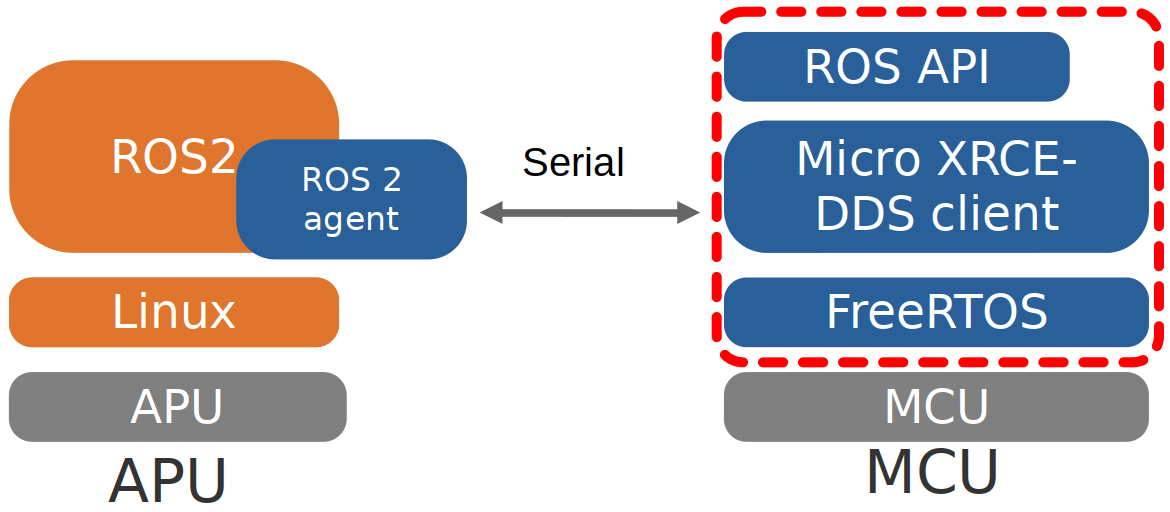
\includegraphics[width=.6\textwidth]{./img/map_microros.png}
\caption{\label{fig:org67a19ab}The FreeRTOS firmware and it's application (red border) are running on the real-time capable side of the Kria CPU. A micro-ROS application is shown here, but any real-time firmware will be deployed in the same way.}
\end{figure}

\subsection{Setting up the IDE}
\label{sec:orgd10f6ea}
Xilinx's Vitis IDE is the recommended tool used to build software for the Xilinx boards.
It also include the tools to interact with the FPGA part, making the whole
software very large (around 200GB of disk usage).

However, this large tool-set allows for a convenient development environment, in particular
in our case where some FreeRTOS system, with many dependencies is to be build.

The installer can be found on \href{https://www.xilinx.com/support/download/index.html/content/xilinx/en/downloadNav/vitis.html}{Xilinx download page}. You will need to get
a file named something like \texttt{Xilinx\_Unified\_2022.2\_1014\_8888\_Lin64.bin}\footnote{The name of the installer binary file might change as a new version of the IDE
is release every year or so.}.

Vitis IDE installer is compatible with versions of Ubuntu, among other distributions,
but not officially yet for the 22.04 version.
Furthermore, the current install was tested on Pop OS, a distribution derived from Ubuntu.
However, even with this more unstable status, no major problems were encountered
with this tool during the development stages.

This guide will present a setup procedure that supposedly works for all distributions based on the newest
LTS from Ubuntu. For other Linux distributions or operating system, please refer to the official documentation.

\subsubsection{Dependencies \& installation}
\label{sec:orga56be12}
Some packages are required to be installed on the host system
in order for the installation process to happen successfully:

\begin{minted}[frame=single,framesep=2mm,baselinestretch=1.2,linenos,breaklines,fontsize=\footnotesize]{sh}
sudo apt-get -y update

sudo apt-get -y install libncurses-dev \
     ncurses-term \
     ncurses-base \
     ncurses-bin \
     libncurses5 \
     libtinfo5 \
     libncurses5-dev \
     libncursesw5-dev
\end{minted}

Once this is done, the previously downloaded binary installer can be executed:

\begin{minted}[frame=single,framesep=2mm,baselinestretch=1.2,linenos,breaklines,fontsize=\footnotesize]{sh}
./Xilinx_Unified_2022.2_1014_8888_Lin64.bin
\end{minted}

If it is not possible to run the previous command, make the file executable with the \texttt{chmod} command:

\begin{minted}[frame=single,framesep=2mm,baselinestretch=1.2,linenos,breaklines,fontsize=\footnotesize]{sh}
sudo chmod +x ./Xilinx_Unified_2022.2_1014_8888_Lin64.bin
\end{minted}

From there you can follow the step-by-step graphical installer.
The directory chosen for the rest of this guide for the Xilinx directory
is directly the \texttt{\$HOME}, but the installation can be set elsewhere is needed.

\begin{tcolorbox}[colback=orange!5!white,colframe=orange!75!black]
\textbf{WARNING}: This whole procedure can take up to multiple hours to complete
and is prone to failures (regarding missing dependencies, typically),
so your schedule should be arranged accordingly.
\end{tcolorbox}

\subsubsection{Platform configuration file generation}
\label{sec:org9632fb8}
In order to have the libraries and configurations in the IDE ready to be used for our board,
we need to obtain some configuration files that are specific for the Kria KV260,
as presented in the \href{https://xilinx.github.io/kria-apps-docs/kv260/2022.1/build/html/docs/build\_vitis\_platform.html?highlight=xsa}{Xilinx guide for Kria and Vitis}.

A Xilinx \href{https://github.com/Xilinx/kria-vitis-platforms}{dedicated repository} is available for us to download  such configurations,
but they required to be built.

As for the dependencies, \texttt{Cmake}, \texttt{tcl} and \texttt{idn} will become needed in order to build the firmware.
Regarding \texttt{idn}, some version issue can happen, but as discussed \href{https://support.xilinx.com/s/question/0D52E00006jrzsYSAQ/platform-project-cannot-be-created-on-vitis?language=en\\\_US}{in a thread on Xilinx's forum},
if \texttt{libidn11} is specifically required but not available (it is the case for Ubuntu 22.04),
creating a symbolic link from the current, 12 version works as a workaround.

Here are the steps for installing the dependencies and building this configuration file:

\begin{minted}[frame=single,framesep=2mm,baselinestretch=1.2,linenos,breaklines,fontsize=\footnotesize]{sh}
sudo apt-get update
sudo apt-get install cmake tcl libidn11-dev \
libidn-dev libidn12 idn
sudo ln -s /usr/lib/x86_64-linux-gnu/libidn.so.12 \
/usr/lib/x86_64-linux-gnu/libidn.so.11

cd ~/Xilinx
git clone --recursive \
https://github.com/Xilinx/kria-vitis-platforms.git
cd kria-vitis-platforms/k26/platforms
export XILINX_VIVADO=/home/$USER/Xilinx/Vivado/2022.2/
export XILINX_VITIS=/home/$USER/Xilinx/Vitis/2022.2/
make platform PLATFORM=k26_base_starter_kit
\end{minted}

\subsection{Setting up and building a new project for the Kria board}
\label{sec:orgf9db271}
With the platform configuration files available, we can now use the IDE to generate a
new project for our board. The whole process will be described with screen captures and
captions.

\begin{figure}[htbp]
\centering
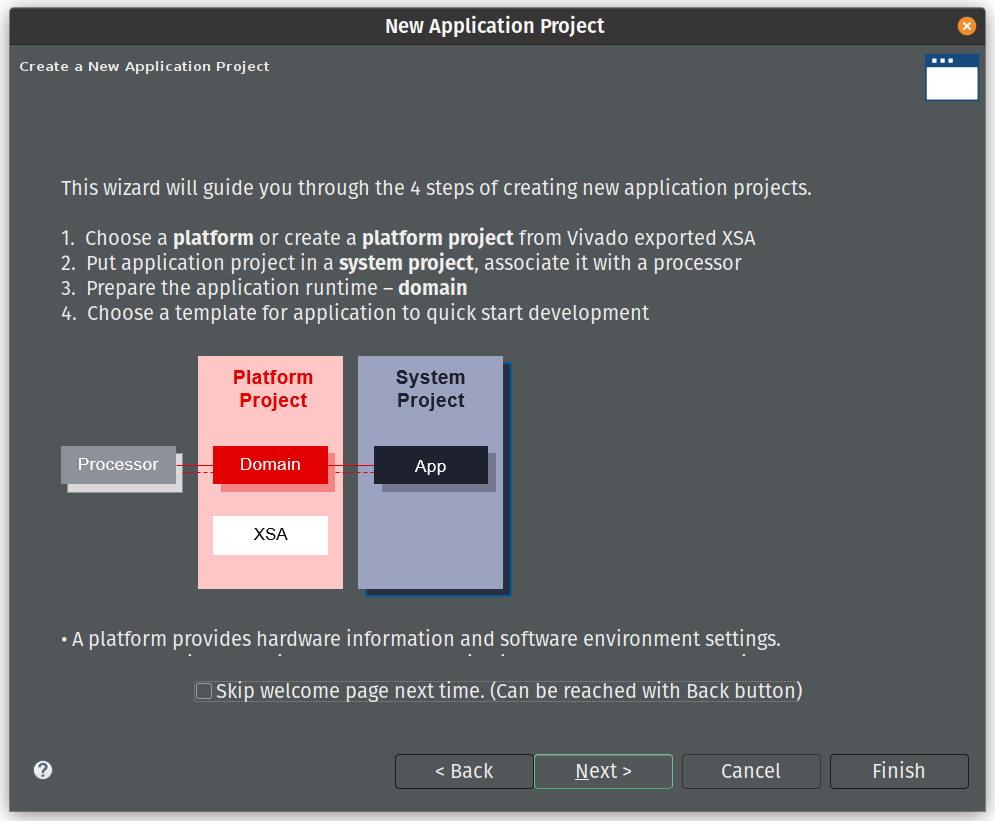
\includegraphics[width=.5\textwidth]{./img/vitis_new/project1.png}
\caption{\label{fig:orgb9eda0a}We are starting with creating a "New Application Project" You should be greeted with this wizard window. Next.}
\end{figure}

\begin{figure}[htbp]
\centering
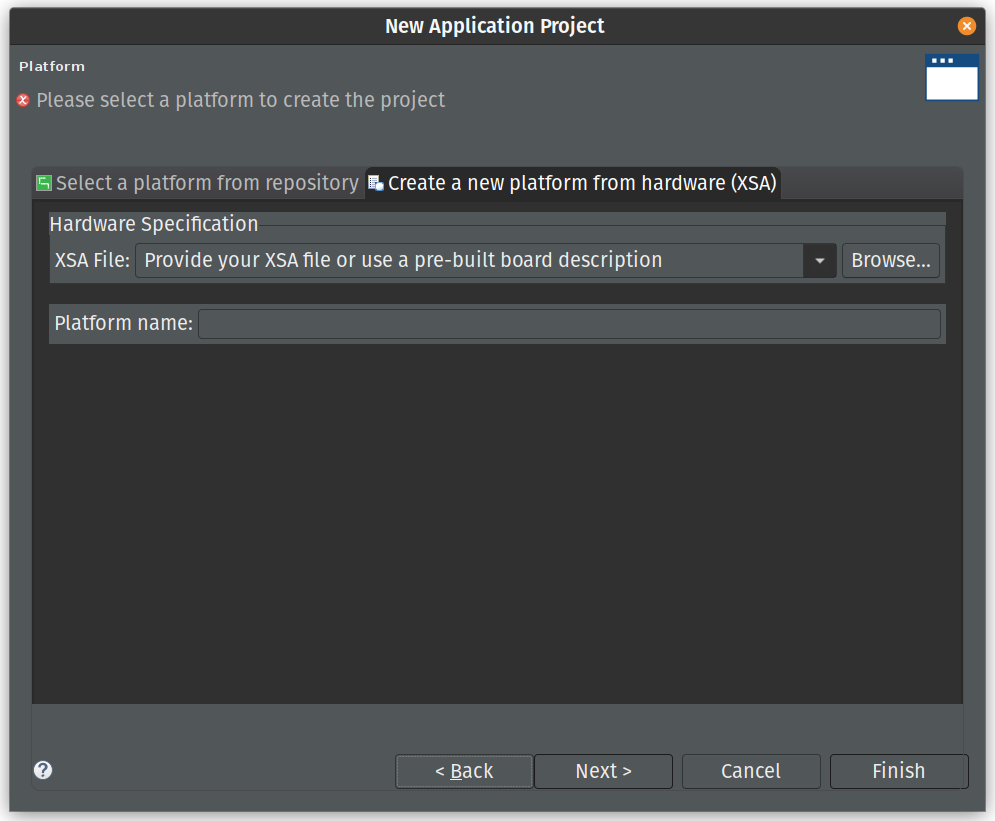
\includegraphics[width=.5\textwidth]{./img/vitis_new/project2.png}
\caption{\label{fig:org580aea3}For the platform, we need to get our build Kria configuration. In the "Create a new platform" tab, click the "Browse\ldots{}" button.}
\end{figure}

\begin{figure}[htbp]
\centering
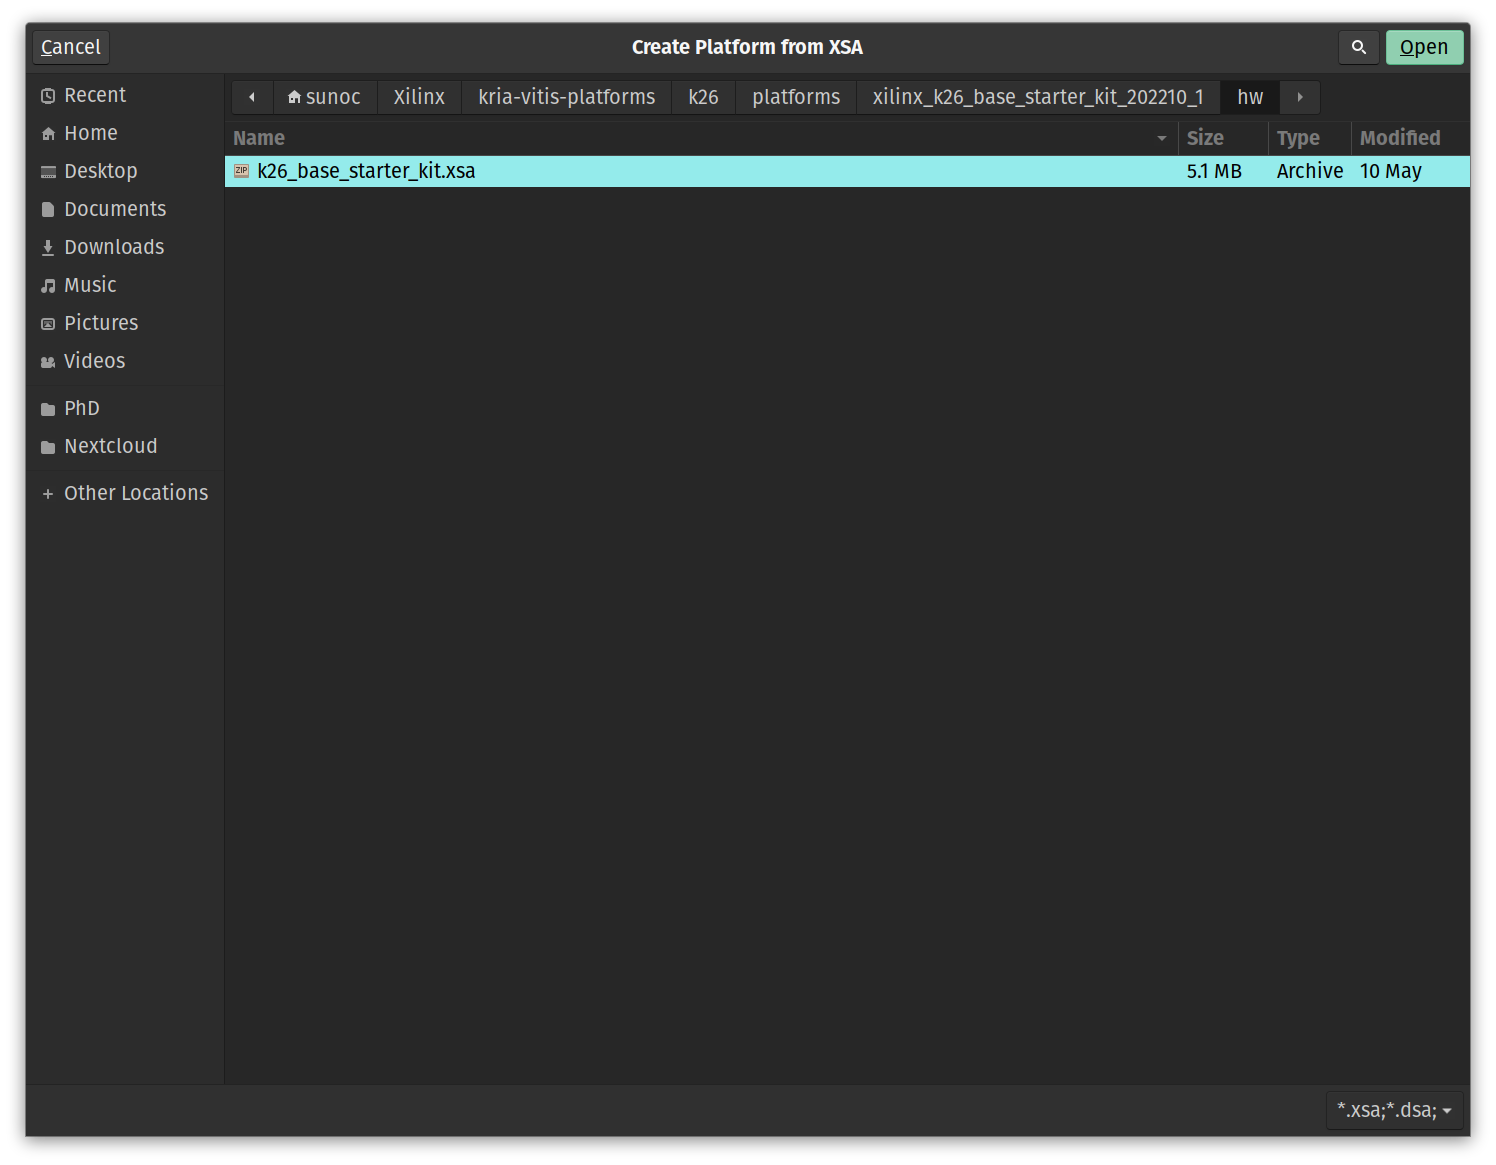
\includegraphics[width=.6\textwidth]{./img/vitis_new/project3.png}
\caption{\label{fig:org341d4d4}In the file explorer, we should navigate in the "k26" directory, where the configuration file was build. From here we are looking for a ".xsa" file, located in a "hw" directory, as visible.}
\end{figure}

\begin{figure}[htbp]
\centering
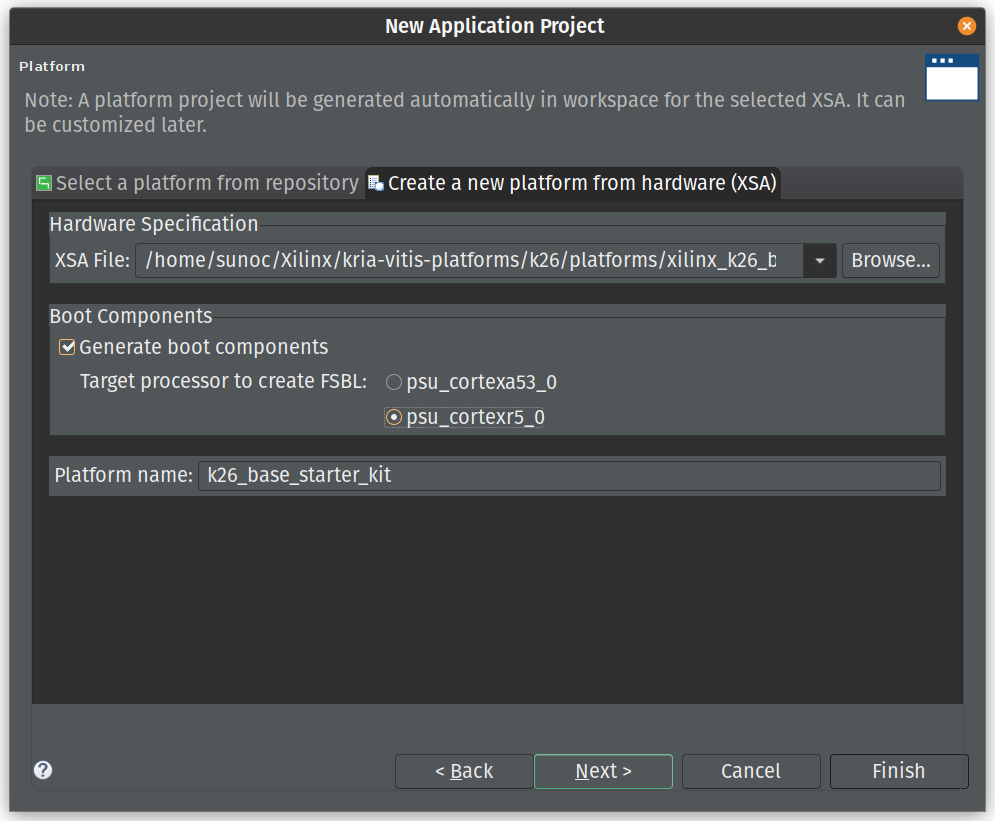
\includegraphics[width=.6\textwidth]{./img/vitis_new/project4.png}
\caption{\label{fig:org18131f8}With the configuration file loaded, we can now select a name for our platform, but most importantly, we have to select the "psu Cortex5 0" core as a target. The other, Cortex 53 is the APU running Linux.}
\end{figure}

\begin{figure}[htbp]
\centering
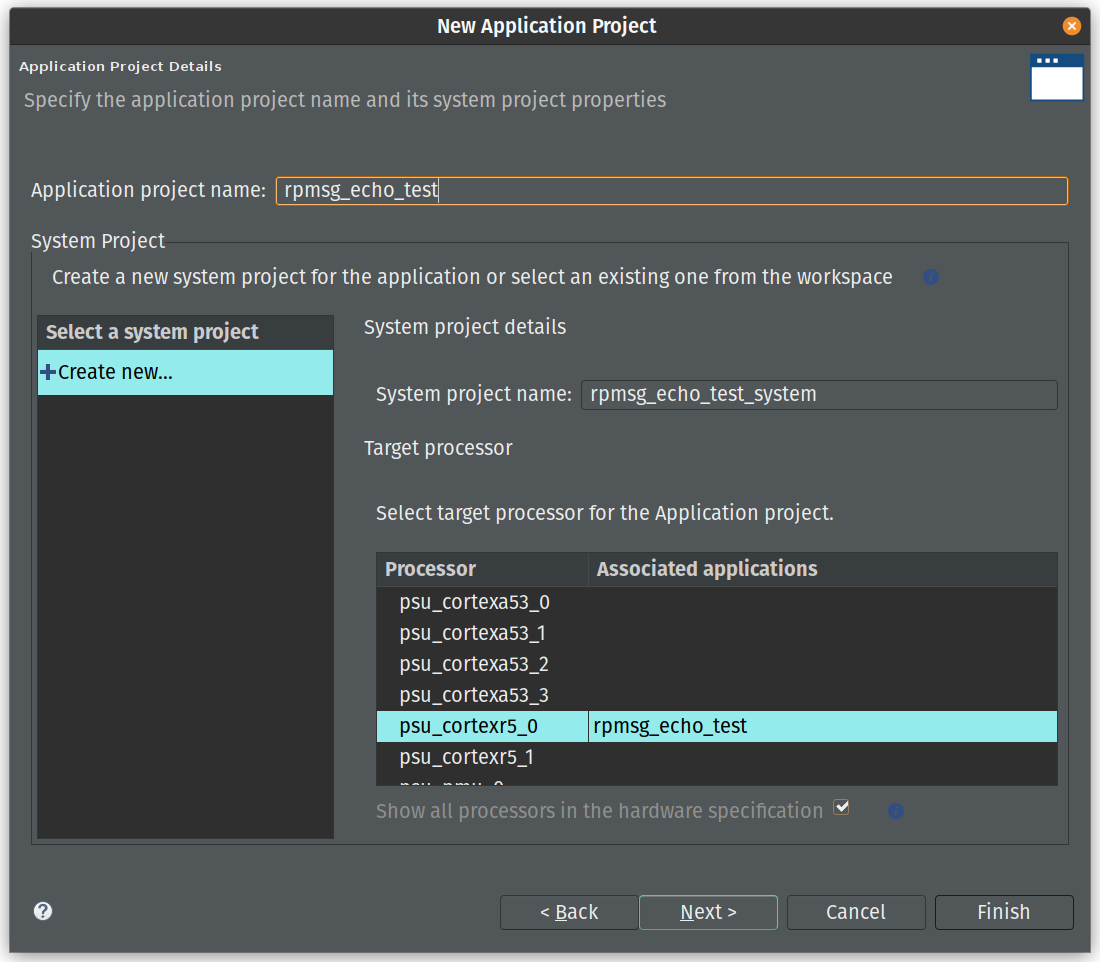
\includegraphics[width=.6\textwidth]{./img/vitis_new/project5.png}
\caption{\label{fig:org5d8cfe4}In this next window, we can give a name to our firmware project. It is also critical here to select the core we want to build for. Once again, we want to use the "psu cortex5 0".}
\end{figure}

\begin{figure}[htbp]
\centering
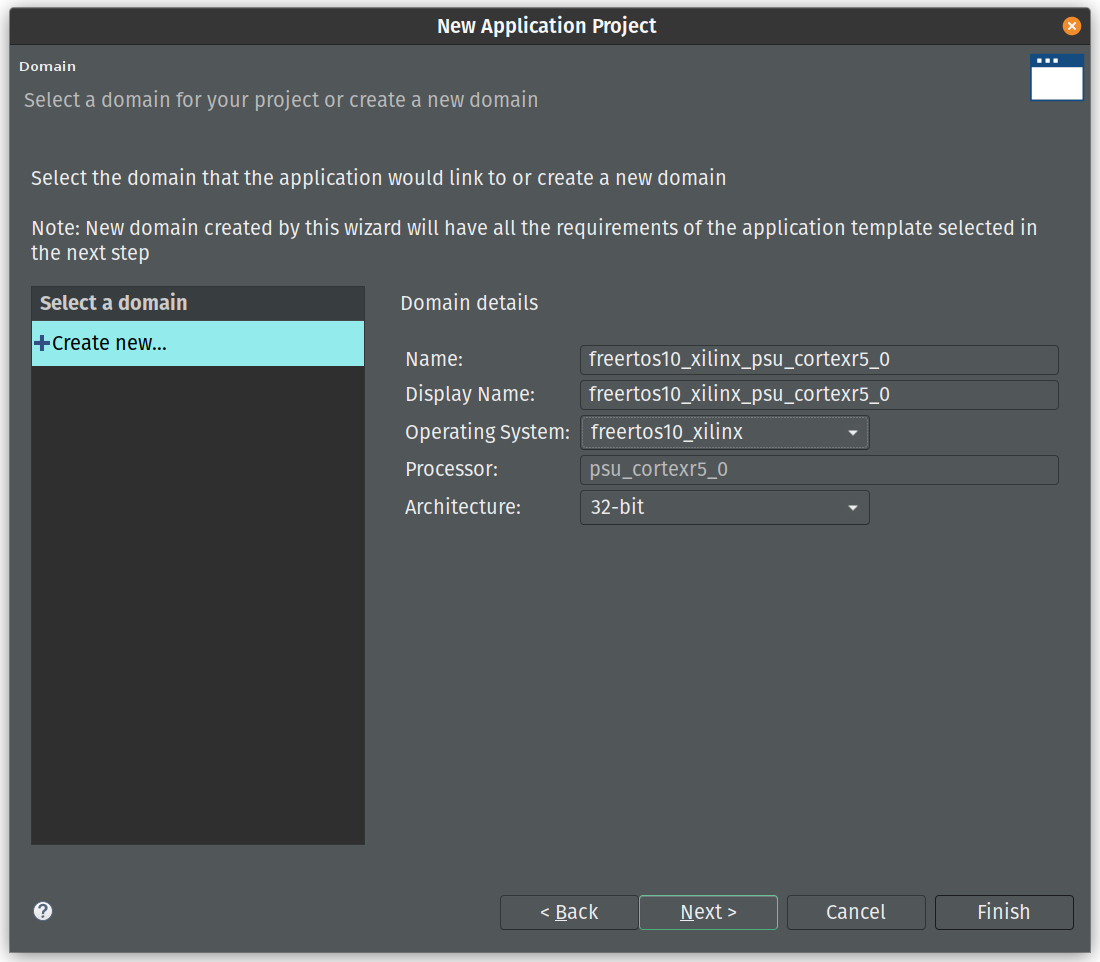
\includegraphics[width=.6\textwidth]{./img/vitis_new/project6.png}
\caption{\label{fig:orgd9cb1d0}Here, we want to select "freertos10 xilinx" as our Operating System. The rest can remain unchanged.}
\end{figure}

\begin{figure}[htbp]
\centering
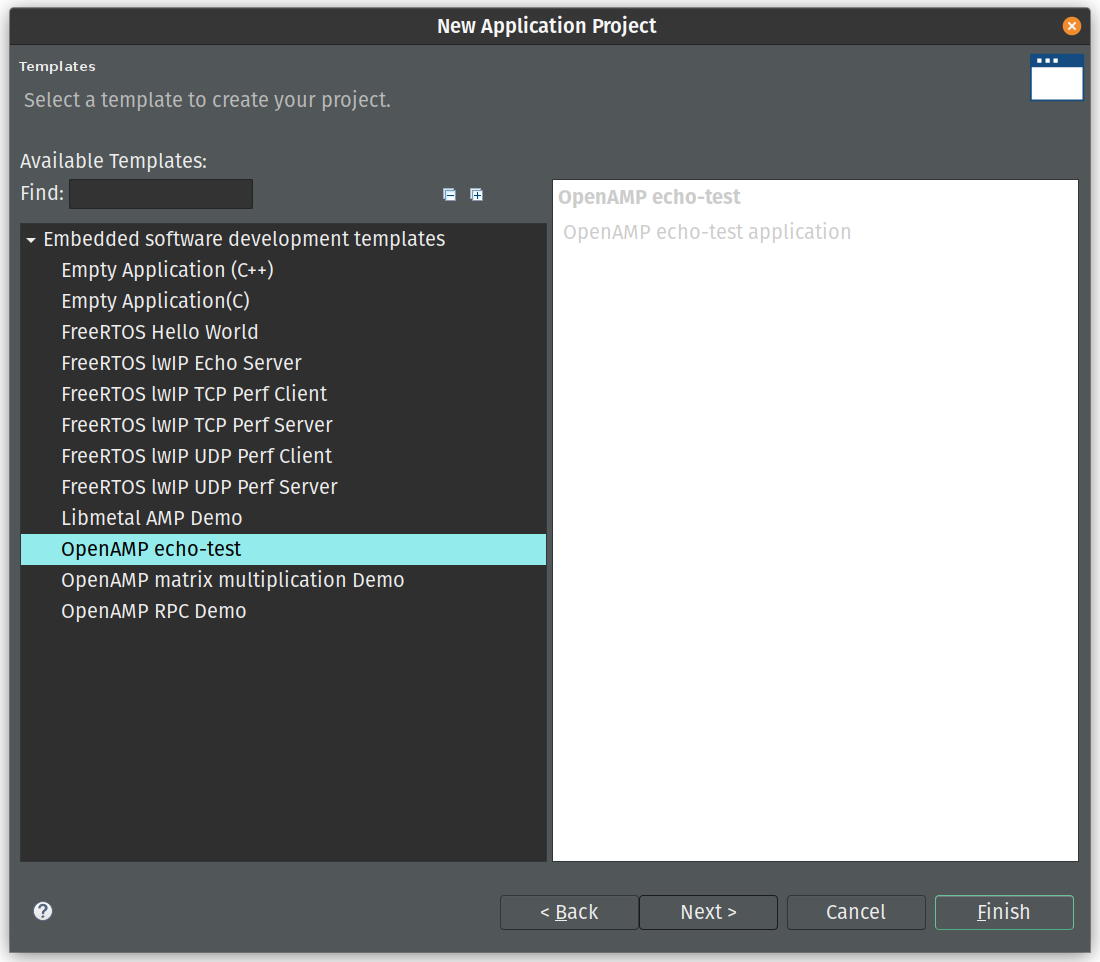
\includegraphics[width=.6\textwidth]{./img/vitis_new/project7.png}
\caption{\label{fig:org5afde50}Finally, we can select the demonstration template we are going to use; here we go with "OpenAMP echo-test" since we want to have some simple try of the RPMsg system. Finish.}
\end{figure}

\pagebreak
In the Xilinx documentation, it is made mention of the addresses setting that should be checked in the \texttt{script.ld} file.
The values in the figure \ref{fig:orge6181e0} below look different from what could be set in the DTO for the Linux side, but they appear to
work for the example we are running, including the new DTO patch without overlapping memory:


\begin{figure}[htbp]
\centering
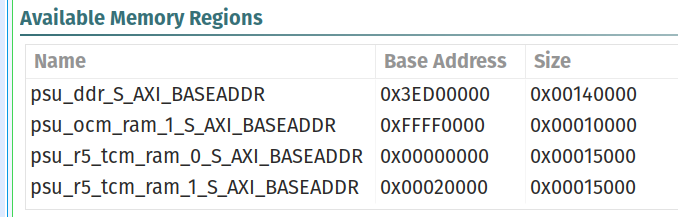
\includegraphics[width=.6\textwidth]{./img/vitis_new/project_mem.png}
\caption{\label{fig:orge6181e0}lscript.ld memory configuration for the firmware memory setup. The same file is available as a whole in this repository's src directory.}
\end{figure}


Once your example project is built and you have a \texttt{.elf} file available, you can
jump directly to the \ref{sec:orgf4d8d82} section to see how to deploy and use your firmware.

The section in between will present setup specifically needed for micro-ROS.

\subsection{Enabling the Stream Buffer system}
\label{sec:org5621e94}
This is a subpart in the general configuration in the project related to some specific
functions for FreeRTOS threads messaging system, however, this point in particular
created so much pain I needed to include in early in this guide for not to forget about it
and keeping a clear track on how to enable this setting.

Indeed, two settings need to be enabled in order to be able to call
functions such as \texttt{xMessageBufferCreate}, useful when working with tasks
in FreeRTOS, as visible in the figure \ref{fig:orgb7b4c37} below:

\begin{figure}[htbp]
\centering
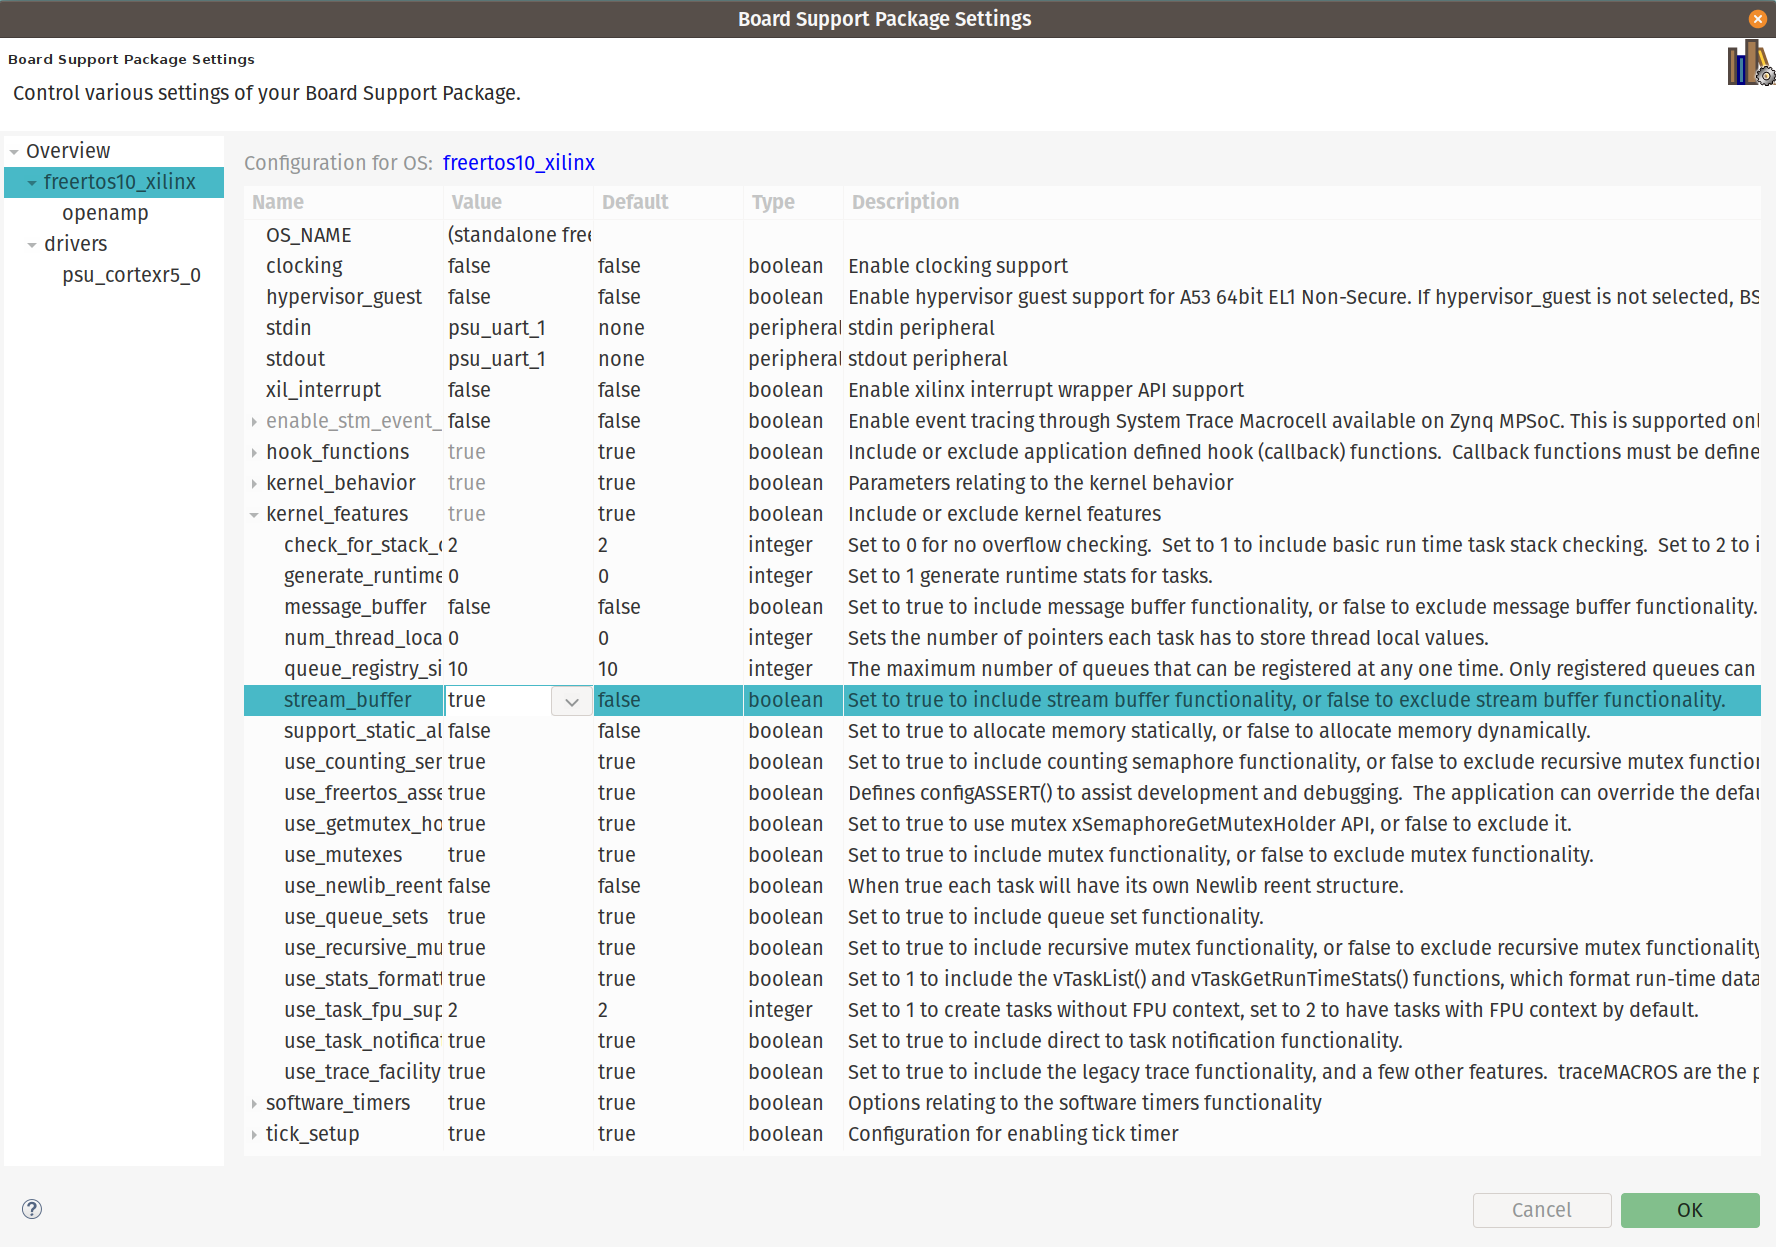
\includegraphics[width=.8\textwidth]{./img/streambuffer.png}
\caption{\label{fig:orgb7b4c37}Enabling Stream Buffer in the Vitis IDE setting: this is a setting that can be found in the "platform.spr" element of your project (the platform, not the firmware project itself). From that file, you can access the settings with the button "Modify BSP Settings", and then as visible, in the tab \texttt{freertos10\_xilinx}, it is needed to toggle here the \texttt{stream\_buffer} setting in the \texttt{kernel\_features}, from the default "false" to "true".}
\end{figure}

\pagebreak
The second setting is useful in the case when a buffer callback function is used, such as\\[0pt]
\texttt{xMessageBufferCreateWithCallback}.
In that case, you must include \texttt{\#define configUSE\_SB\_COMPLETED\_CALLBACK 1} on the top of you header
file (in our project, this will happen in the \texttt{microros.h} header file),
before the \texttt{\#include "FreeRTOS.h"} in order to override the setting from this include.


\pagebreak
\section{RPMsg \texttt{echo\_test} software}
\label{sec:org0a0cccf}
In order to test the deployment of the firmware on the R5F side, and in particular
to test the RPMsg function, we need some program on the Linux side of the Kria
board to "talk" with the real-time side.

Some source is provided by Xilinx to build a demonstration software that does
this purpose: specifically interact with the demonstration firmware.

Here are the steps required to obtain the sources, and build the program.

As a reminder, this is meant to be done on the Linux running on the
Kria board, NOT on your host machine !

\begin{minted}[frame=single,framesep=2mm,baselinestretch=1.2,linenos,breaklines,fontsize=\footnotesize]{sh}
git clone https://github.com/Xilinx/meta-openamp.git
cd  meta-openamp
git checkout xlnx-rel-v2022.2
cd  ./recipes-openamp/rpmsg-examples/rpmsg-echo-test
make
sudo ln -s $(pwd)/echo_test /usr/bin/
\end{minted}

Once this is done, it it possible to run the test program from the Kria board's Ubuntu
by running the \texttt{echo\_test} command.

\section{Building micro-ROS as a static library}
\label{sec:org05184c8}
In this section, the goal is to build the micro-ROS library in order to be
able to integrate it's functions into our Cortex R5F firmware.

All of this should be done via cross-compiling on a host machine, however
it is most common in the guides about micro-ROS to build the firmwares and libraries within a Docker,
so we can have access of the ROS environment without installing it permanently.

One can simply run this command to summon a ROS2 Docker\footnote{If Docker is not set up on your machine, you can follow the guide on \href{https://docs.docker.com/engine/install/ubuntu/}{the official website}.
When you can successfully run the "hello-world" container, you are good to go.} with the wanted version,
but first we also need to check the cross-compilation tools.

We are downloading the latest \texttt{arm-none-eabi} gcc compiler directly from the ARM website.

The cross-compilation tool can then be extracted, set as our \texttt{toolchain} variable,
then passed as a parameter when creating the Docker container:
\begin{minted}[frame=single,framesep=2mm,baselinestretch=1.2,linenos,breaklines,fontsize=\footnotesize]{sh}
pushd /home/$USER/Downloads
wget https://developer.arm.com/-/media/Files/downloads/\
gnu/12.2.mpacbti-rel1/binrel/arm-gnu-toolchain-12.2\
.mpacbti-rel1-x86_64-arm-none-eabi.tar.xz
tar -xvf arm-gnu-toolchain-12.2.mpacbti-rel1-x86_64-\
arm-none-eabi.tar.xz
popd

toolchain="/home/$USER/Downloads/arm-gnu-toolchain-\
12.2.mpacbti-rel1-x86_64-arm-none-eabi/"


docker run -d --name ros_build -it --net=host \
--hostname ros_build \
-v /dev:/dev \
-v $toolchain:/armr5-toolchain \
--privileged ros:iron
\end{minted}

Now the container named \texttt{ros\_build} was created, it is possible to "enter" it, and having access
to the tools in it by running the following command that will open a \texttt{bash} shell in said container:
\begin{minted}[frame=single,framesep=2mm,baselinestretch=1.2,linenos,breaklines,fontsize=\footnotesize]{sh}
docker exec -it ros_build bash
\end{minted}

Now we are in the ROS2 container, we can build the micro-ROS firmware as presented
in the \href{https://micro.ros.org/docs/tutorials/advanced/create\\\_custom\\\_static\\\_library}{dedicated micro-ROS guide}:
\begin{minted}[frame=single,framesep=2mm,baselinestretch=1.2,linenos,breaklines,fontsize=\footnotesize]{sh}
sudo apt update 
sudo apt-get -y install python3-pip \
     wget \
     nano

. /opt/ros/\$ROS_DISTRO/setup.bash

mkdir microros_ws
cd microros_ws
git clone -b \$ROS_DISTRO \
    https://github.com/micro-ROS/micro_ros_setup.git \
    src/micro_ros_setup

sudo rosdep fix-permissions &&\
    rosdep update &&\
    rosdep install --from-paths src --ignore-src -y

colcon build
. ./install/local_setup.bash

ros2 run micro_ros_setup create_firmware_ws.sh generate_lib
\end{minted}

From that point, we will need some extra configuration files for our Cortex R5F.

Both configuration files\footnote{Both files are also visible in the appendixes \ref{sec:org90c1115}
and \ref{sec:orgd236854} the end of this report.\}} will be downloaded from my repository;
we also are going to copy the cross-compiler into the microros workspace,
then we can build the library with the following ros2 command:
\begin{minted}[frame=single,framesep=2mm,baselinestretch=1.2,linenos,breaklines,fontsize=\footnotesize]{sh}
wget https://gitlab.com/sunoc/xilinx-kria-kv260-\
documentation/-/raw/main/src/custom_r5f_toolchain.cmake

wget https://gitlab.com/sunoc/xilinx-kria-kv260-\
documentation/-/raw/main/src/custom_r5f_colcon.meta

cp -r /armr5-toolchain/ \$(pwd)/firmware/toolchain && \
export PATH=\$PATH:\$(pwd)/firmware/toolchain/bin

ros2 run micro_ros_setup build_firmware.sh \
\$(pwd)/custom_r5f_toolchain.cmake \$(pwd)/\
custom_r5f_colcon.meta
\end{minted}
\pagebreak

\section{Including micro-ROS to the real-time firmware}
\label{sec:org6048d69}
Now we have a Vitis demonstration project available and the \texttt{libmicroros} static library
available, we can combine both by including this library into our Kria project.

On the host machine running the IDE, we can download the static library
and the include files from the Docker builder.
Here, we assume your Vitis IDE workspace sits in you home directory, at \texttt{\textasciitilde{}/workspace},
and that the Docker container is named \texttt{ros\_build}:
\begin{minted}[frame=single,framesep=2mm,baselinestretch=1.2,linenos,breaklines,fontsize=\footnotesize]{sh}
mkdir /home/$USER/workspace/microros_lib

docker cp ros_build:/microros_ws/firmware/build/\
       libmicroros.a /home/$USER/workspace/microros_lib/

docker cp ros_build:/microros_ws/firmware/build/include \
       /home/$USER/workspace/microros_lib/
\end{minted}

Many parameters are available to be set up in the IDE for the compilation toolchain, but
the figures \ref{fig:org1f78872} and \ref{fig:org8066ecd} below will show you a setup that worked to have the IDE
to recognize the include files and to be able to use them for compiling the firmware.

\begin{figure}[htbp]
\centering
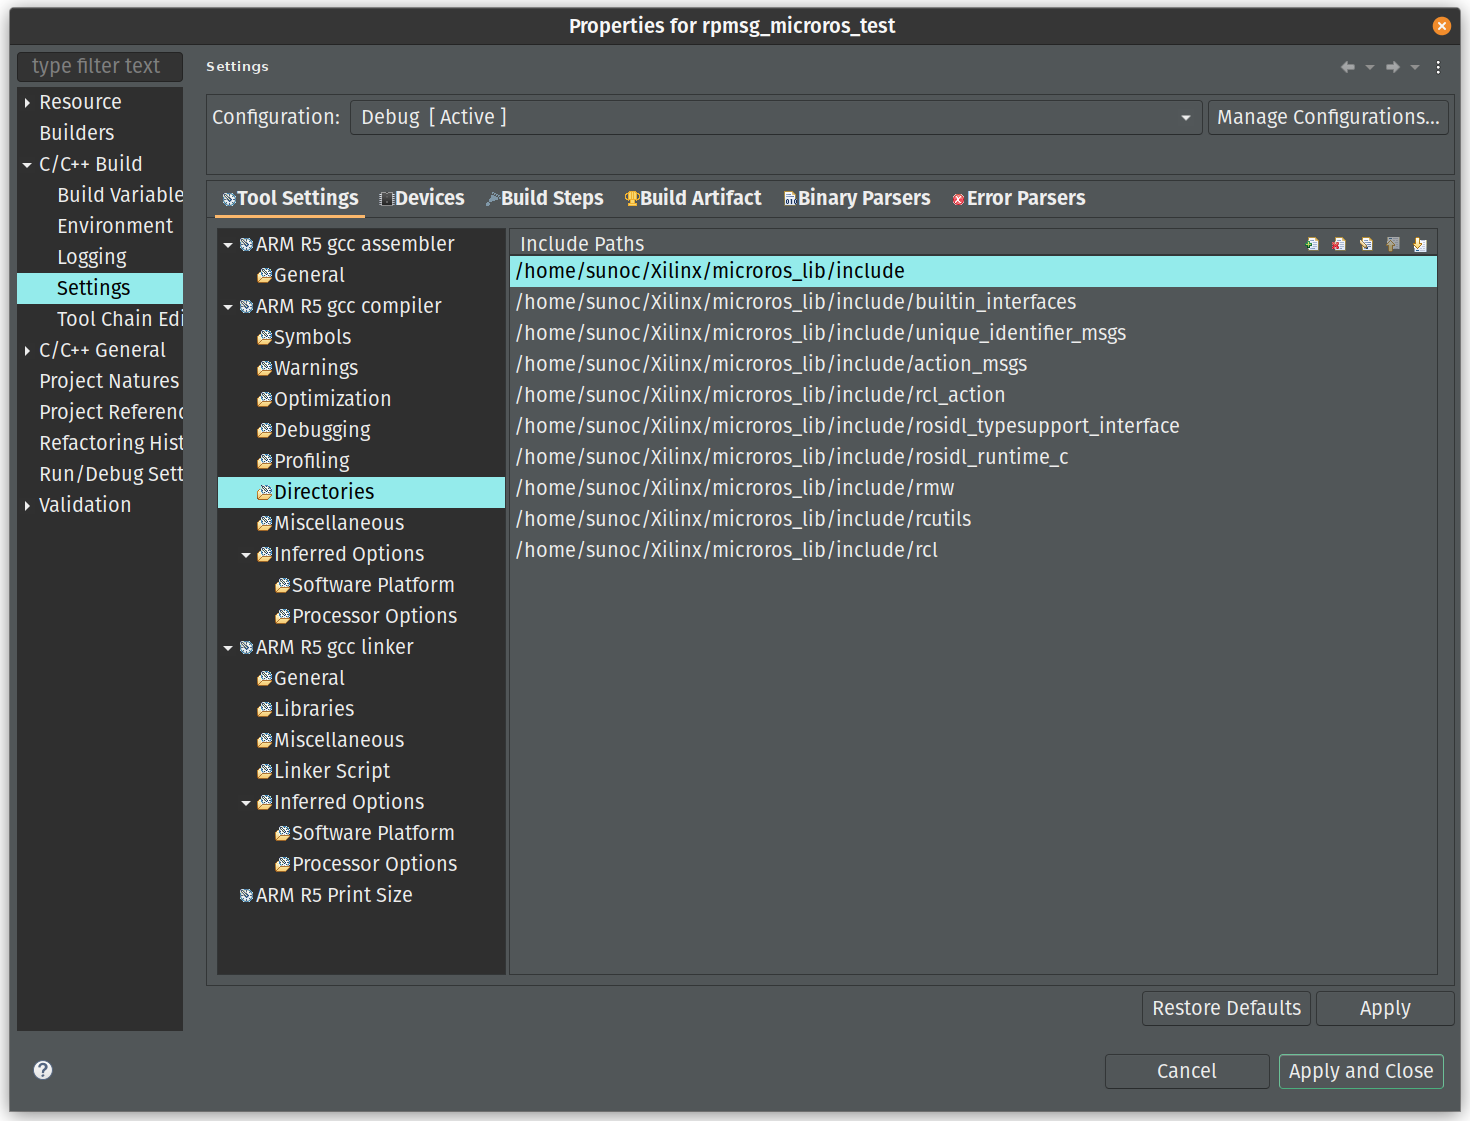
\includegraphics[width=.8\textwidth]{./img/vitis_new/include.png}
\caption{\label{fig:org1f78872}Firstly, in the "C/C++ Build" settings of your firmware project, under the "Settings" menu, you should find the gcc compiler "Directories". In here you should add the "include" directory of your library. Be careful however, if your include files are in a second layer of directory (as it is the case for libmicroros) you will need to include each sub-directory individually, as visible in this figure.}
\end{figure}

\begin{figure}[htbp]
\centering
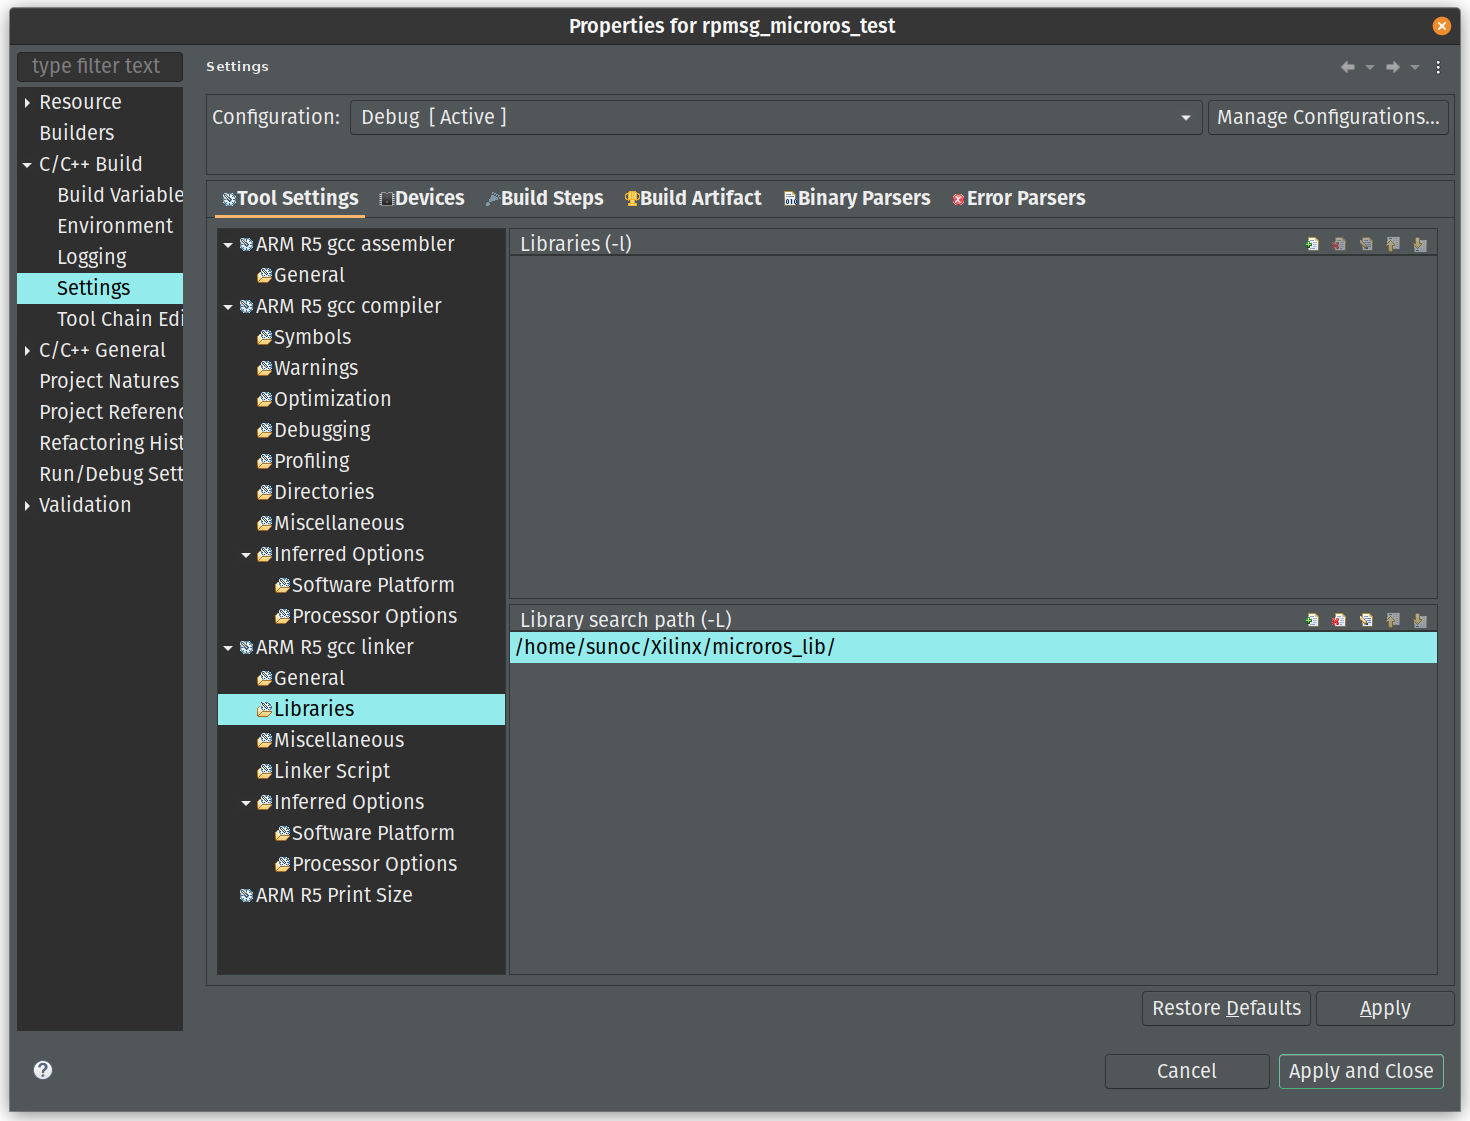
\includegraphics[width=.8\textwidth]{./img/vitis_new/include2.png}
\caption{\label{fig:org8066ecd}Secondly, in the gcc linkers "Libraries", you can add the top level directory of your library. In our case, it is the directory that contains both the "include" directory added earlier, and also the "libmicroros.a" file.}
\end{figure}

\pagebreak
With both of these setup in your project and as a minimal test to see if the setup was made correctly,
you should be able to include the following micro-ROS libraries into your project:
\begin{minted}[frame=single,framesep=2mm,baselinestretch=1.2,linenos,breaklines,fontsize=\footnotesize]{c}
#include <rcl/rcl.h>
#include <rcl/error_handling.h>
#include <rclc/rclc.h>
#include <rclc/executor.h>
\end{minted}

The details for the inclusions and the use-case of the library will depend on the implementation
of the firmware itself.

But in general, as the firmware is successfully built and an \texttt{.elf} file is available and can be uploaded as a
firmware to the Kria board (or any remote server accessible through \texttt{SSH}, for that matter) with the following
command\footnote{Note that in that case, we are retrieving the binary for a project
named \texttt{rpmsg\_pingpong\_microros\_lib}.
You own path will vary depending on how your project was named in the first place.
Obviously, the \texttt{SSH} connection parameters will also be specific to your case.
The \texttt{ubuntu@192.168.1.10} set here are merely an example.}:
\begin{minted}[frame=single,framesep=2mm,baselinestretch=1.2,linenos,breaklines,fontsize=\footnotesize]{sh}
scp /home/sunoc/workspace/rpmsg_pingpong_microros_lib/\
    Debug/rpmsg_pingpong_microros_lib.elf  ubuntu@192.168.1.10:/home/ubuntu/
\end{minted}
\pagebreak

\section{micro-ROS adaptation for the firmware}
\label{sec:org9d813b7}
Beyond the inclusion of the library itself, actually using the micro-ROS system
within an external project require more than just importing the needed
functions.

Indeed, if you would be just adding the various function for sending messages to
the general ROS2 network, you would face issues with four key aspects.
These are presented in the following dedicated sub-sections.

\subsection{Time functions}
\label{sec:org8665218}
As micro-ROS can be used on a variety of board, it does not understand by itself
what time functions are meant to be used.

In that regard, some API-style function are being
used in the library and it is then needed for the person using a new board
to implement these function inner working using the board own time-related
function calls.

In particular for this part, the \texttt{clock\_gettime} function is key, and could
simply be implemented with some FreeRTOS time functions.

The end result for these implementation are visible in the appendix \ref{sec:org773176c},
and can be reused as-if for the Kria board setups.

\subsection{Memory allocators}
\label{sec:orgd0ada2a}
Similarly to the time function, it is required to re-implement some form of memory allocating
functions in order for the library to be able to work with such functions in a formalized way.

As for now, the current version of the allocator function can be seen in the
appendix \ref{sec:org0e9dade}, but the current setup is not
completely "clean", some further formatting, test and modification will be needed.

\subsection{Custom transport layer\hfill{}\textsc{WORK\_IN\_PROGRESS}}
\label{sec:org96df670}
This part is the key translation layer that needs to happen in order for the
DDS system from the micro-ROS library to be using the communication channel we
want it to.

A problem that we had to figure out lives in the fact that the operation of micro-ROS DDS
and the board's RPMsg communication system does not operate in the same fashion.

The former expects to have four functions ("open", "read", "write" and "close") that can
be called and used by the main system, while the latter relies on FreeRTOS callback
system, waiting on the service interrupt routine to be trigger by an incoming message.

This situation meant that we count not simple translate the communication layers from one
to another: a non-blocking polling and buffer system needed to be put into places.
The proposed solution that was implemented and that is currently being tested
is showed and detailed in the figure \ref{fig:orgce3f64d} below.

As this part of the firmware was developed and tested on it's own, the overall
implementation within the "real" ping-pong application is still a work in progress,
and further modifications are expected when the system will be more thoroughly tested.

\begin{figure}[htbp]
\centering
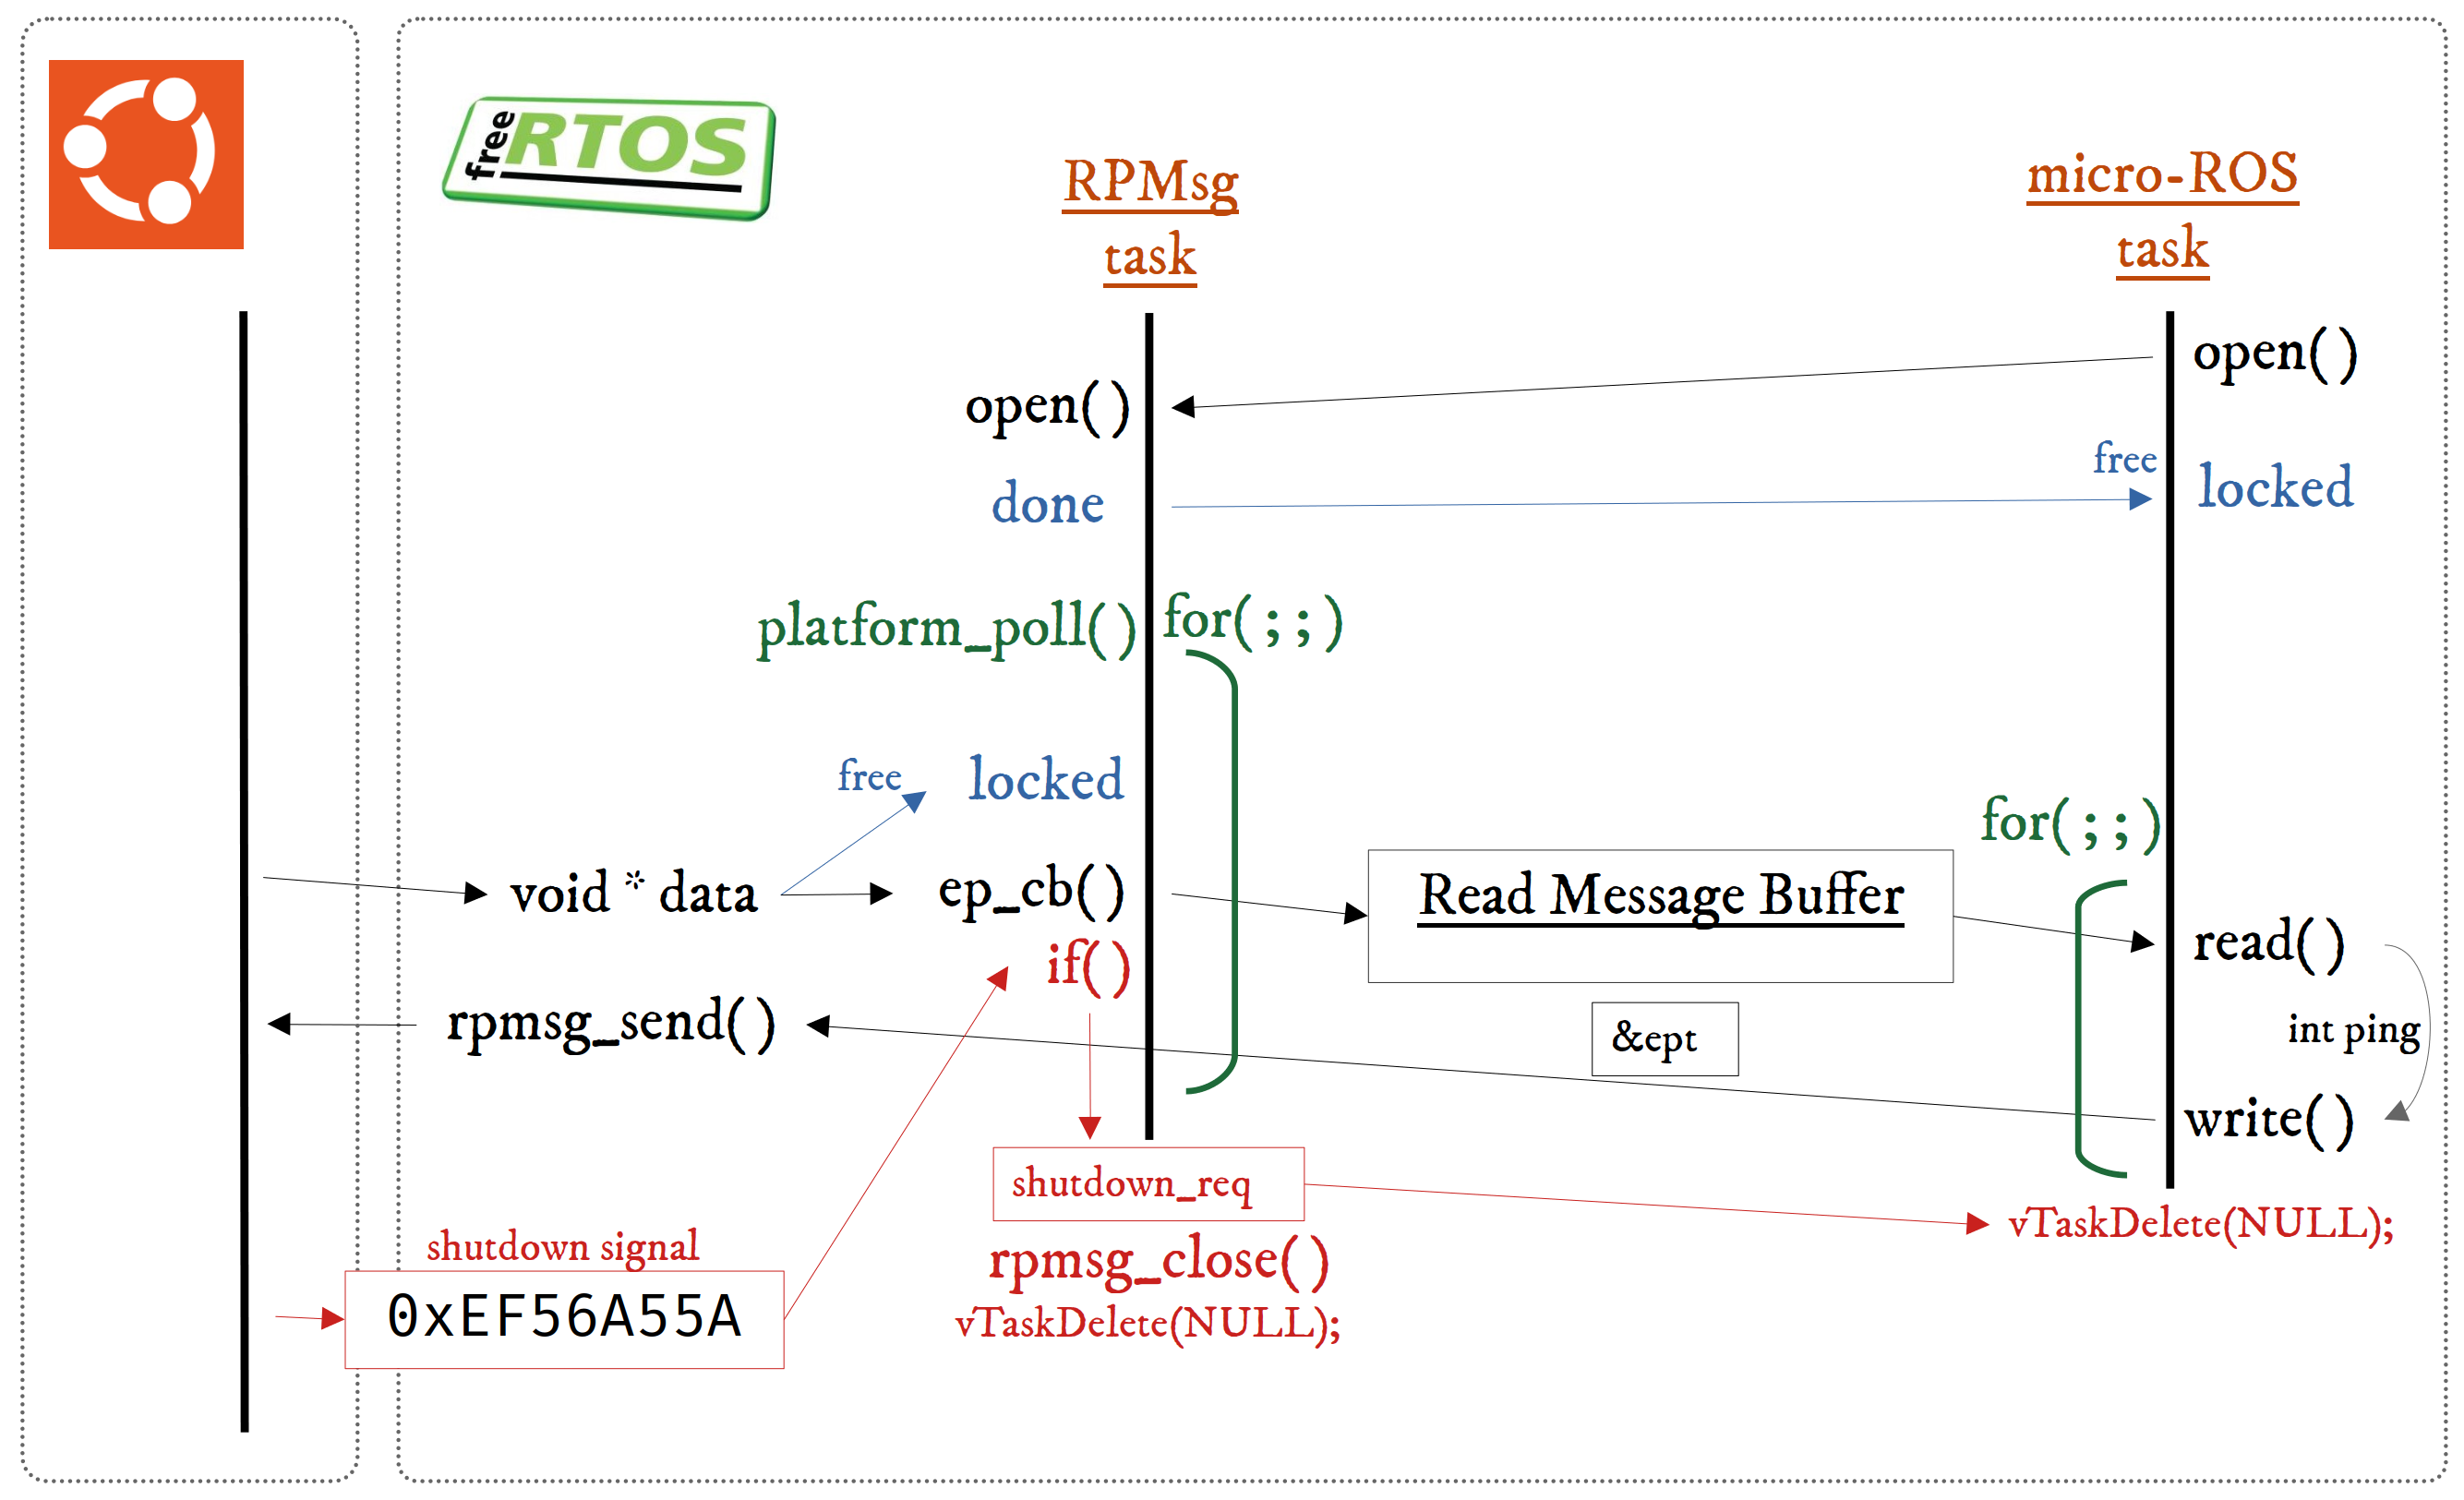
\includegraphics[width=1\textwidth]{./img/rpmsg_fw_tasks.png}
\caption{\label{fig:orgce3f64d}Two tasks are being run concurrently in order to manage the communication situation, with binary semaphore-based lock-unlock system.\\[0pt]
 The role of the micro-ROS task (right) is to make the four functions ("open", "read", "write" and "close")  available and running the actual software function. In this example, polling the read function and writing back when something is receive (ping-pong function). The use of the \texttt{rpmsg\_send()} function is done directly from the micro-ROS task, bypassing the RPMsg task in this situation.\\[0pt]
 In the libmicroros implementation currently being developed, the micro-ROS task holds all the DDS and micro-ROS system, including the mentioned allocators function.\\[0pt]
 The RPMsg task (center) is used to firstly set the RPMsg communication with the Linux side (left), then it stays locked until the ISR (interrupt service routine) is triggered by an incoming message. The message is then passed to the micro-ROS task using a buffer.\\[0pt]
 When a shutdown signal is received from the Linux, both functions will gracefully close and are getting killed.}
\end{figure}

\pagebreak
\section{Loading the firmware}
\label{sec:orgf4d8d82}
Having a version of our \texttt{.elf} firmware (with or without the included
micro-ROS library) built and loaded onto our Kria's Linux, we want to load and run it
on the Cortex micro-controller side.

As a reminder, the firmware can be loaded from the host machine IDE workspace
to the Kria board through \texttt{SSH} using the following command:
\begin{minted}[frame=single,framesep=2mm,baselinestretch=1.2,linenos,breaklines,fontsize=\footnotesize]{sh}
scp /home/sunoc/workspace/rpmsg_pingpong_microros_lib/\
    Debug/rpmsg_pingpong_microros_lib.elf  ubuntu@192.168.1.10:/home/ubuntu/
\end{minted}

The following instructions will show how to use this binary file, and
in particular how to upload and start the firmware on the R5F real time core
from the Linux user-space\footnote{In this sequence, we are entering a root shell with \texttt{sudo -s}, but this can
also be archived by putting the commands in a script to be executed with \texttt{sudo}.}, to test a basic RPMsg setup\footnote{It is also important to note that the \texttt{echo\_test} part is specific for the
RPMsg base demonstration firmware. It is not to be used for other firmware.
The instruction to build and use this particular program on the Kria Linux
is visible in the section \ref{sec:org0a0cccf}.}:
\begin{minted}[frame=single,framesep=2mm,baselinestretch=1.2,linenos,breaklines,fontsize=\footnotesize]{sh}
sudo -s
mv image_echo_test /lib/firmware
echo image_echo_test  > /sys/class/remoteproc/\
     remoteproc0/firmware
echo start > /sys/class/remoteproc/remoteproc0/state
echo_test
echo stop > /sys/class/remoteproc/remoteproc0/state
\end{minted}

In this setup you need to be careful for the name of the \texttt{.elf} binary to be exactly used
in the first \texttt{mv} and \texttt{echo} command. In this example, the binary would be named
\texttt{image\_echo\_test.elf}, and moved from \texttt{\$HOME} to \texttt{/lib/firmware}.

The debug of the firmware itself is done by reading the "printf" visible from the serial
return of the board (typically a \texttt{/dev/ttyUSB1}), but two things are to be noted:
\begin{itemize}
\item If the \texttt{echo start} command fails, either the previous firmware run was not stopped,
or the new binary itself is impossible to run.
\item In general, if the \texttt{echo\_test} runs, it means that everything is okay and that
the RPMsg system worked successfully.
\end{itemize}
\pagebreak


\section{Running a ROS2 node}
\label{sec:orgc9d4b3a}
This section as well as the next one are rather "separated" from the rest of the report, as
they are focused on the ROS2 system being used on the Kria board.

In this first section, the installation of ROS2 as a system will be presented, with
two different ways of approaching the problem.

As for the previous section, the figure \ref{fig:orgd75c38a} below shows what part
of the overall system we are talking about here.

\begin{figure}[htbp]
\centering
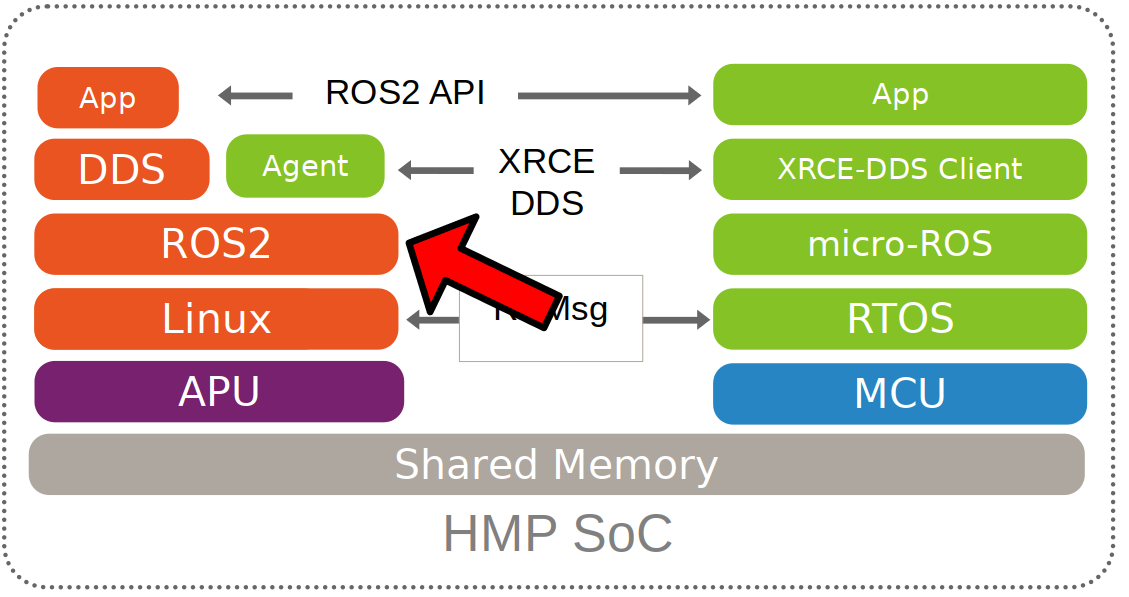
\includegraphics[width=.6\textwidth]{./img/map_ros.png}
\caption{\label{fig:orgd75c38a}The ROS2 middle (red border) runs on top of the Linux, on the general-purpose core of the Kria board.}
\end{figure}

\subsection{On the host Linux ("bare-metal")}
\label{sec:orgde4cb5f}
Since an Ubuntu distribution is installed on the board, the installation of ROS2
can be done\footnote{As always, this configuration was tested solely on Ubuntu LTS 22.04,
with the ROS2 versions \texttt{Humble} and then \texttt{Iron} being deployed.
Other combination of versions should work as well, but they are not
tested for this guide. In case of doubt or problem, please refer to the official documentation.} in a standard way, using the repository.

An \href{https://docs.ros.org/en/humble/Installation/Ubuntu-Install-Debians.html}{official documentation} is provided with ROS2 themselves with a step-by-step guide on how to install
ROS2 on a Ubuntu system\{\}.
We will be following this guide here\footnote{The \texttt{curl} command from the guide does not work through the school proxy,
but the command \texttt{wget} used instead does work. The key is then moved to the correct spot with \texttt{mv}.}.

Firstly, we need to update the locals, enable the universe Ubuntu repository,
get the key and add the repository for ROS2. This can be done as follow:
\begin{minted}[frame=single,framesep=2mm,baselinestretch=1.2,linenos,breaklines,fontsize=\footnotesize]{sh}
locale  # check for UTF-8
sudo apt update && sudo apt install -y locales
sudo locale-gen en_US en_US.UTF-8
sudo update-locale LC_ALL=en_US.UTF-8 LANG=en_US.UTF-8
export LANG=en_US.UTF-8
locale  # verify settings

sudo apt install -y software-properties-common
sudo add-apt-repository universe
sudo apt update && sudo apt install -y curl wget

wget https://raw.githubusercontent.com/ros/rosdistro/master/ros.key
sudo mv ros.key /usr/share/keyrings/ros-archive-keyring.gpg
\end{minted}

Then, a thicc one-liner is available to add the ROS2 repository to our system:
\begin{minted}[frame=single,framesep=2mm,baselinestretch=1.2,linenos,breaklines,fontsize=\footnotesize]{sh}
echo "deb [arch=$(dpkg --print-architecture) \
signed-by=/usr/share/keyrings/ros-archive-keyring.gpg] \
http://packages.ros.org/ros2/ubuntu $(. \
/etc/os-release && echo $UBUNTU_CODENAME) main" | \
sudo tee /etc/apt/sources.list.d/ros2.list > /dev/null
\end{minted}

It is then possible to install ROS2\footnote{This command installs a complete "desktop" version of ROS2, containing many
useful package for our project.
If space is a constraint, different, less complete packages can be install.
Please refer to the official documentation about it.} as follow:
\begin{minted}[frame=single,framesep=2mm,baselinestretch=1.2,linenos,breaklines,fontsize=\footnotesize]{sh}
sudo apt update
sudo apt upgrade -y
sudo apt install -y ros-humble-desktop \
     ros-humble-ros-base \
     python3-argcomplete \
     ros-dev-tools
\end{minted}

Once installed, it is possible to test the system with a provided example.
You need to open two terminals and log wish SSH onto the board, then running
respectively:
\begin{minted}[frame=single,framesep=2mm,baselinestretch=1.2,linenos,breaklines,fontsize=\footnotesize]{sh}
source /opt/ros/humble/setup.bash
ros2 run demo_nodes_cpp talker
\end{minted}

And then:
\begin{minted}[frame=single,framesep=2mm,baselinestretch=1.2,linenos,breaklines,fontsize=\footnotesize]{sh}
source /opt/ros/humble/setup.bash
ros2 run demo_nodes_py listener
\end{minted}

You should be able to see the first terminal sending "Hello world" messages,
and the second one receiving then.

\subsection{In a container (Docker)}
\label{sec:org8da44bc}
As containers are used to test and build micro-ROS configurations,
running ROS2 in a Docker  is a great way to have a reproducible configuration
of you system.

This part of the guide will present how to install Docker on the
Kria board and then how to use it to deploy the latest version of ROS2.

\subsubsection{Installing Docker on Ubuntu}
\label{sec:orgdae867e}
It is possible to have a version of Docker installed simply by using the available repository,
but since we are on Ubuntu, a PPA is available from Docker in order to have the most up-to-date version.

Following \href{https://docs.docker.com/engine/install/ubuntu/\#install-using-the-repository}{the official documentation}, the following steps can be taken to install the latest version of
Docker on a Ubuntu system. The last command is meant to test the install.
If everything went smoothly, you should see something similar to what is presented
in the figure \ref{fig:org71d6e8b} below, after the commands:

\begin{minted}[frame=single,framesep=2mm,baselinestretch=1.2,linenos,breaklines,fontsize=\footnotesize]{sh}
sudo apt-get update
sudo apt-get install ca-certificates curl sudo
gnupg install -m 0755 -d /etc/apt/keyrings
curl -fsSL https://download.docker.com/linux/ubuntu/gpg | \
    sudo gpg --dearmor -o /etc/apt/keyrings/docker.gpg

sudo chmod a+r /etc/apt/keyrings/docker.gpg

echo \
    "deb [arch="$(dpkg --print-architecture)" \
  signed-by=/etc/apt/keyrings/docker.gpg] \
  https://download.docker.com/linux/ubuntu \
  "$(. /etc/os-release && \
         echo "$VERSION_CODENAME")" stable" | \
    sudo tee /etc/apt/sources.list.d/docker.list > /dev/null

sudo apt-get update
sudo apt-get install docker-ce docker-ce-cli \
     containerd.io docker-buildx-plugin docker-compose-plugin
sudo usermod -aG docker $USER
newgrp docker

docker run hello-world
\end{minted}

\begin{figure}[htbp]
\centering
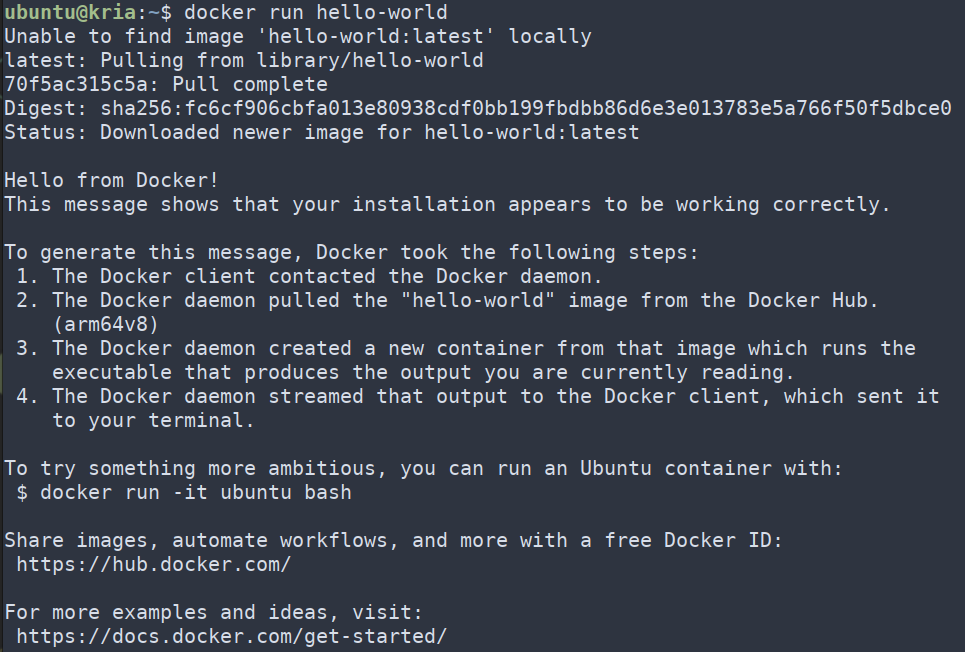
\includegraphics[width=.7\textwidth]{./img/hello-docker.png}
\caption{\label{fig:org71d6e8b}The return of a successful run of the \texttt{hello world} test Docker container.}
\end{figure}


\subsubsection{Running a ROS2 container}
\label{sec:org0a105e7}
The following commands will pull a ROS container, version \texttt{iron}, and name it \texttt{ros\_build}.

A key part for having access to the interfaces (serial) is the mapping of the whole \texttt{/dev}
range of devices from the host machine to the internal \texttt{/dev} of the container\footnote{This is an example and this situation can become a security issue. It would be a better practice
in a production environment to map only the devices that are actually in use.}.
With the second command, we can execute \texttt{bash} as a way to open a terminal to the "inside" the container:
\begin{minted}[frame=single,framesep=2mm,baselinestretch=1.2,linenos,breaklines,fontsize=\footnotesize]{sh}
docker run -d --name ros_agent -it --net=host -v \
       /dev:/dev --privileged ros:iron
docker exec -it ros_agent bash
\end{minted}

From there, it becomes possible to simply use ROS2 as you would for a bare-metal install,
and as presented in the section \ref{sec:orgde4cb5f} above:
\begin{minted}[frame=single,framesep=2mm,baselinestretch=1.2,linenos,breaklines,fontsize=\footnotesize]{sh}
source /opt/ros/$ROS_DISTRO/setup.bash

# Create a workspace and download the micro-ROS tools
mkdir microros_ws
cd microros_ws
git clone -b $ROS_DISTRO https://github.com/micro-ROS/\
    micro_ros_setup.git src/micro_ros_setup

# Update dependencies using rosdep
sudo apt update && rosdep update
rosdep install --from-paths src --ignore-src -y

# Install pip
sudo apt-get install python3-pip

# Build micro-ROS tools and source them
colcon build

# Download micro-ROS-Agent packages
source install/local_setup.bash
ros2 run micro_ros_setup create_agent_ws.sh

# Build step
ros2 run micro_ros_setup build_agent.sh

# Run a micro-ROS agent
ros2 run micro_ros_agent micro_ros_agent serial \
     --dev /dev/ttyUSB1
\end{minted}

Then once again in a similar way to the bare-metal deployment,  it is possible to run a demonstration
the ping-pong topic communication from a different shell\footnote{You need to be careful to have you shell in the "correct" space: these command need to be run inside
the container in which the previous setup were install, not on the host running the container system.
The hostname should help you to figure out where you are.}:
\begin{minted}[frame=single,framesep=2mm,baselinestretch=1.2,linenos,breaklines,fontsize=\footnotesize]{sh}
source /opt/ros/$ROS_DISTRO/setup.bash

# Subscribe to micro-ROS ping topic
ros2 topic echo /microROS/ping
\end{minted}
\pagebreak


\section{micro-ROS agent\hfill{}\textsc{WORK\_IN\_PROGRESS}}
\label{sec:org95c1378}
The micro-ROS agent on the ROS2 side is the last piece of the puzzle needed to
allow our DDS environment to use RPMsg as a mean of communication, as visible
on the schematic of the figure \ref{fig:orgecf24f9} below.
In particular, it will be useful to modify this agent in order to archive
the full RPMsg communication for ROS2\footnote{This will be done with ROS2 agents "custom transport"  system,
which has little documentation. Some \href{https://github.com/micro-ROS/micro\_ros\_setup/issues/383}{discussions} about it exist though.}.
An \href{https://micro.ros.org/docs/tutorials/advanced/create\_custom\_transports/}{official documentation} exists, but it gives little to no detail
on how to deploy such modified, custom transport setup.
This part of the guide will focus on it.

\begin{figure}[htbp]
\centering
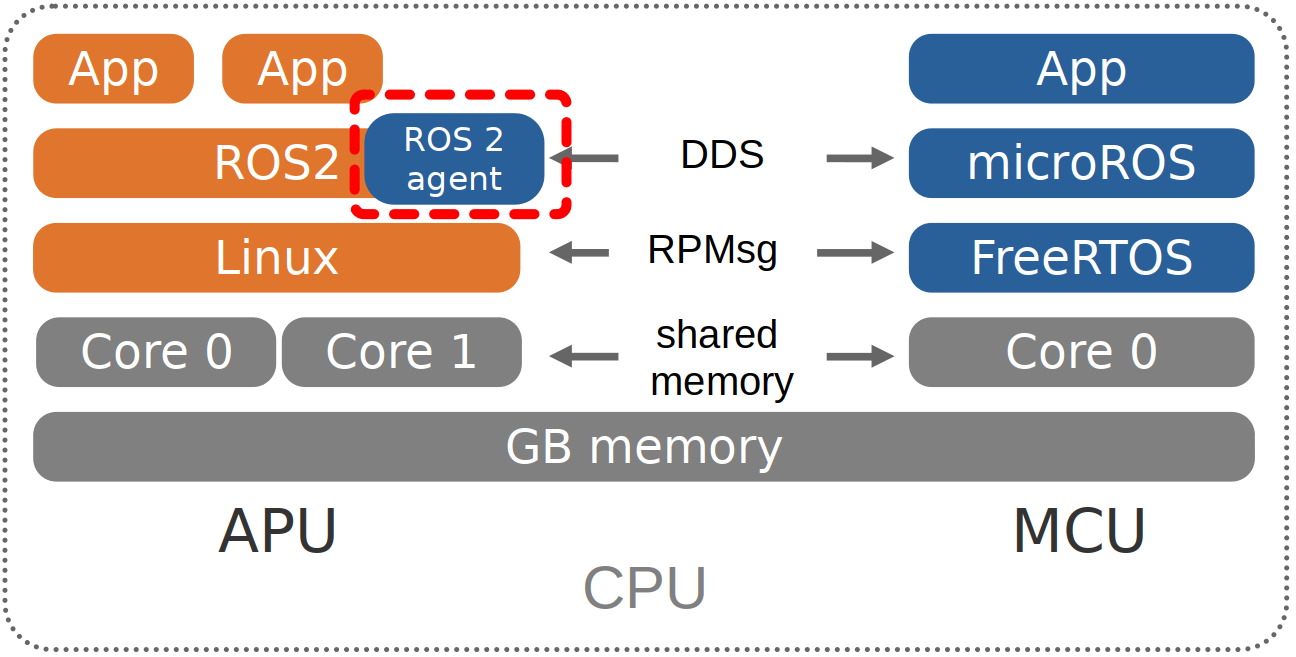
\includegraphics[width=.6\textwidth]{./img/map_agent.png}
\caption{\label{fig:orgecf24f9}The agent (red border) allows for a micro-ROS instance to communicate with a ROS2 system. It is deployed on the Linux side, as a ROS2 node.}
\end{figure}


\subsection{Building a eProsima agent bare-metal}
\label{sec:orgb0e56ca}
A key aspect to understand about modifying the agent (as
this will be needed later on to support our new communication system),
is that the default system and instruction provided by micro-ROS does not
allow such modification\footnote{This information was eventually found on a discussion in a \href{https://github.com/micro-ROS/micro\_ros\_setup/issues/591}{GitHub Issue thread}.}.

In order to avoid that, one can get and run a ROS2 node design by eProsima,
that can be deployed on it's own (without other ROS2 application and nodes)
and eventually modified.


\begin{minted}[frame=single,framesep=2mm,baselinestretch=1.2,linenos,breaklines,fontsize=\footnotesize]{sh}
sudo nano /microros_ws/build/micro_ros_agent/agent/src/xrceagent/src/cpp/transport/custom/CustomAgent.cpp
\end{minted}
The same file is available online as a reference, on \href{https://github.com/eProsima/Micro-XRCE-DDS-Agent/blob/develop/src/cpp/transport/custom/CustomAgent.cpp}{eProsima XRCE-DDS-Agent GitHub repository}.


\begin{minted}[frame=single,framesep=2mm,baselinestretch=1.2,linenos,breaklines,fontsize=\footnotesize]{sh}
git clone https://github.com/eProsima/Micro-XRCE-DDS-Agent.git
cd Micro-XRCE-DDS-Agent/

rm -rf examples/
git clone https://gitlab.com/sunoc/rpmsg-micro-ros-agent.git ./examples/custom_agent

mkdir build && cd build
cmake -DUAGENT_BUILD_USAGE_EXAMPLES=ON ..
make
\end{minted}

The custom agent is then available to run from the \texttt{./src/examples/custom\_agent/CustomXRCEAgent}.

All the diff when the custom agent system was added:
\url{https://github.com/eProsima/Micro-XRCE-DDS-Agent/pull/205/files}

For rebuilding the custom agent with a simple \texttt{make clean \&\& make all} will
conveniently only rebuild the part that was modify.
Which means that once all the libraries have been compiled once,
the subsequent re-compilation of the agent itself can be done quickly !

Major details on how to implement a custom agent specified here:
\url{https://github.com/eProsima/Micro-XRCE-DDS-Agent/issues/195\#issuecomment-721002153}


\subsection{Building the XRCE-DDS agent in a Docker}
\label{sec:orgf37b4a8}
The same command presented above for running a custom agent "bare-metal" can be
run inside a Docker.

\begin{minted}[frame=single,framesep=2mm,baselinestretch=1.2,linenos,breaklines,fontsize=\footnotesize]{sh}
docker run -d --name XRCE_DDS_Agent -it --net=host -v \
       /dev:/dev --privileged ros:iron
docker exec -it XRCE_DDS_Agent bash
\end{minted}


\begin{minted}[frame=single,framesep=2mm,baselinestretch=1.2,linenos,breaklines,fontsize=\footnotesize]{sh}
git clone https://github.com/eProsima/Micro-XRCE-DDS-Agent.git
cd Micro-XRCE-DDS-Agent
docker build -t xrce-dds-agent .
docker run -it --privileged -v /dev:/dev xrce-dds-agent serial \
       --dev /dev/ttyACM0
\end{minted}


\subsection{Creating a custom transport agent}
\label{sec:org5d67420}


\pagebreak


\section{Conclusion \& future\hfill{}\textsc{WORK\_IN\_PROGRESS}}
\label{sec:orge6562dc}

\pagebreak
\appendix


\section{DTO patch}
\label{sec:org3406614}
This file is available in this repository: \href{https://gitlab.com/sunoc/xilinx-kria-kv260-documentation/-/blob/b7300116e153f4b5a1542f8804e4646db8030033/src/system.patch}{system.patch}
\inputminted[linenos, frame=single]{diff}{./src/system.patch}

\pagebreak
\section{Custom toolchain CMake settings}
\label{sec:org90c1115}
This file is available in this repository: \href{https://gitlab.com/sunoc/xilinx-kria-kv260-documentation/-/blob/b7300116e153f4b5a1542f8804e4646db8030033/src/custom\_r5f\_toolchain.cmake}{custom r5f toolchain.cmake}
\inputminted[linenos, frame=single]{cmake}{./src/custom_r5f_toolchain.cmake}

\pagebreak
\section{Custom Colcon meta settings}
\label{sec:orgd236854}
This file is available in this repository: \href{https://gitlab.com/sunoc/xilinx-kria-kv260-documentation/-/blob/b7300116e153f4b5a1542f8804e4646db8030033/src/custom\_r5f\_colcon.meta}{custom r5f colcon.meta}
\inputminted[linenos, frame=single]{yaml}{./src/custom_r5f_colcon.meta}

\pagebreak
\section{Firmware time functions}
\label{sec:org773176c}

\subsection{main}
\label{sec:orgad9f244}
This file is available in this repository: \href{https://gitlab.com/sunoc/xilinx-kria-kv260-documentation/-/blob/b7300116e153f4b5a1542f8804e4646db8030033/src/clock.c}{clock.c}
but a potentially more up-to-date version is visible
directly at the \texttt{libmicroros\_kv260} repository: \href{https://gitlab.com/sunoc/libmicroros\_kv260/-/blob/4867e762f66af7b4647232eb4c0a31106db66e13/src/clock.c}{clock.c}

\inputminted[linenos, frame=single]{c}{./src/clock.c}

\subsection{header file}
\label{sec:org8e1f510}
\begin{minted}[frame=single,framesep=2mm,baselinestretch=1.2,linenos,breaklines,fontsize=\footnotesize]{c}
/**< Microseconds per second. */
#define MICROSECONDS_PER_SECOND    ( 1000000LL )  
/**< Nanoseconds per second. */
#define NANOSECONDS_PER_SECOND     ( 1000000000LL ) 
/**< Nanoseconds per FreeRTOS tick. */  
#define NANOSECONDS_PER_TICK       ( NANOSECONDS_PER_SECOND / configTICK_RATE_HZ ) 
\end{minted}


\pagebreak
\section{Firmware memory allocation functions}
\label{sec:org0e9dade}

\subsection{main}
\label{sec:org9ec5510}
This file is available in this repository: \href{https://gitlab.com/sunoc/xilinx-kria-kv260-documentation/-/blob/b7300116e153f4b5a1542f8804e4646db8030033/src/allocators.c}{allocators.c}
but a potentially more up-to-date version is visible
directly at the \texttt{libmicroros\_kv260} repository: \href{https://gitlab.com/sunoc/libmicroros\_kv260/-/blob/4867e762f66af7b4647232eb4c0a31106db66e13/src/allocators.c}{allocators.c}

\inputminted[linenos, frame=single]{c}{./src/allocators.c}

\subsection{header file}
\label{sec:org718c7fd}
\begin{minted}[frame=single,framesep=2mm,baselinestretch=1.2,linenos,breaklines,fontsize=\footnotesize]{c}
#ifndef _ALLOCATORS_H_
#define _ALLOCATORS_H_

#include "microros.h"

extern int absoluteUsedMemory;
extern int usedMemory;


void * __freertos_allocate(size_t size, void * state);
void __freertos_deallocate(void * pointer, void * state);
void * __freertos_reallocate(void * pointer, size_t size, void * state);
void * __freertos_zero_allocate(size_t number_of_elements,
size_t size_of_element, void * state);

#endif // _ALLOCATORS_H_
\end{minted}
\end{document}